\documentclass[a4paper,12pt]{article}
\usepackage{textcomp}
\usepackage{amssymb}
\usepackage{gensymb}
\usepackage{array}
\usepackage{booktabs}
\usepackage{tabularx}
\usepackage{supertabular}
\usepackage{longtable}
\usepackage{graphicx}
\usepackage{float}
\usepackage{placeins}
\usepackage{pgfplots}
\pgfplotsset{compat=1.7}
\parindent=0pt
\usepackage{xurl}
\usepackage{amsmath}
\numberwithin{equation}{section}
\usepackage[margin=2.5cm]{geometry}
\usepackage[utf8]{inputenc}
\usepackage{nomencl}
\makenomenclature
\usepackage{float}
\usepackage{subfig}
\usepackage{breakcites}
\usepackage{graphicx}
\graphicspath{{images/}}
\emergencystretch=1em
\setcounter{page}{1}
\usepackage{float}
\usepackage{xcolor}
\renewcommand{\baselinestretch}{1.5}
\usepackage{titlesec}
\usepackage{hyperref}
\setcounter{secnumdepth}{4}
\titleformat{\paragraph}
{\normalfont\normalsize\bfseries}{\theparagraph}{1em}{}
\titlespacing*{\paragraph}
{0pt}{3.25ex plus 1ex minus .2ex}{1.5ex plus .2ex}
\usepackage{amsmath}
\numberwithin{figure}{section}
\hypersetup{
    colorlinks=false,
    pdfborder={0 0 0},
    pdftitle={THE INVESTIGATION OF GRAPHENE AND ITS UTILISATION IN FLEXIBLE DISPLAYS},}
    
\begin{document}

%TC:ignore
\begin{titlepage}
\begin{center}

{\Large{THE INVESTIGATION OF GRAPHENE AND ITS UTILISATION IN FLEXIBLE DISPLAYS}}
\vspace{08cm}

\Large{By Khushnood Asif}

\vspace{10cm}

\Large{DEN318 Third Year Project (Mech) April 2021}

\Large{Supervisor:  Dr PATRICK CULLEN }

\vspace{6cm}

\cleardoublepage
\thispagestyle{empty}
{\Large{SCHOOL OF ENGINEERING AND MATERIALS SCIENCE}}
\vspace{1cm}

\Large{ENGINEERING/MATERIALS}

\Large{THIRD YEAR PROJECT}

\Large{DEN318}

\vspace{1cm}



{\Large{\textbf{DECLARATION}}}
\vspace{3cm}
\end{center}

\noindent This report entitled
\vspace{1cm}
\begin{center}
    \textbf{ THE INVESTIGATION OF GRAPHENE AND ITS UTILISATION IN FLEXIBLE DISPLAYS }
\end{center}
\vspace{1cm}
Was composed by me and is based on my own work. Where the work of the others
has been used, it is fully acknowledged in the text and in captions to table
illustrations. This report has not been submitted for any other qualification.


\vspace{2cm}

{\Large \textbf{Name}: \ \ \ Khushnood Asif}
\vspace{1cm}

{\Large \textbf{Signed: \ 
\includegraphics[height=1.2\baselineskip]{signature}}}
\vspace{1cm}

{\Large \textbf{Date:} \ \ \ \ \ 28/04/2021}
\end{titlepage}

\cleardoublepage

\pagenumbering{roman}
\begin{abstract}
\pagenumbering{roman}

\noindent Graphene can have numerous advantages in mobile phone displays. There are currently 14.02 billion mobile devices globally, which is expected to rise to 17.72 billion devices by 2024 (Statista, 2020). The number of mobile devices is twice as high as the number of people (7.8 billion). More than 90\% of the mobile phone display market is made from a transparent conductive material called Indium Tin Oxide (ITO). It has both high electrical conductivity and high optical transparency. However, mobile phones suffer from factors that affect their performance and quality, such as brittleness, so they tend to break or smash when dropped. ITO is a finite material with its own set of difficulties, including rising prices (costing \$1020 per kg - (Sigma-Aldrich, 752657)) and difficulty mining because of depletion. A global market for ITO is \$1.57 billion per year with an expected growth rate (360researchreports.com, 2020). Therefore, replacing ITO presents a huge market opportunity. This project aims to conduct a literature review and simulate and model the materials listed in the literature designed to replace ITO used in mobile screens. A graphene-based composite can serve as a suitable replacement for ITO. (Asif, 2020)

\end{abstract}
\pagebreak
\vspace{1cm}

\newpage
\tableofcontents

\newpage


\nomenclature[1]{$\theta$}{Bending Angle (degrees)}
\nomenclature[2]{I}{Imposed Displacement (mm)}
\nomenclature[3]{L}{Length of the Screen (mm)}
\nomenclature[4]{P}{Load (N)}
\nomenclature[5]{$\upsilon$}{Poisson's Ratio (no units)}
\nomenclature[6]{$\sigma$}{Tensile Strength (MPa)}
\nomenclature[7]{W}{Width of the Screen (mm)}
\nomenclature[8]{$E$}{Young's Modulus (MPa)}

\makeatletter
     \renewcommand*\l@figure{\@dottedtocline{1}{1em}{3.2em}}
\makeatother
\listoffigures
\phantomsection
\addcontentsline{toc}{section}{List of Figures}
\newpage
\listoftables
\phantomsection
\addcontentsline{toc}{section}{List of Tables}
\newpage
\printnomenclature
\phantomsection
\addcontentsline{toc}{section}{Nomenclature}
%TC:endignore


\newpage
\section{Introduction}
\pagenumbering{arabic}

\subsection{Background}

\noindent Demand for display technologies is increasing, driving research to transform devices such as mobile phones. A flexible, transparent, and foldable display is necessary to meet consumer demands for convenience and efficiency. Mechanically, displays should be able to react to repeated bending and flexing. But conventional displays are usually fabricated on brittle electrodes such as indium in oxide (ITO), which have poor mechanical strain tolerance. Therefore, alternatives that are flexible and transparent have been studied to replace ITO. (Lee, 2020)\vspace{\baselineskip}

\noindent Graphene has excellent electrical, optical, and mechanical properties, making it an ideal candidate for use in display devices. It is an interesting material and is an enigma since it is commonly believed to be a laboratory product.\vspace{\baselineskip}

\begin{figure}[H]
  \centering
  \begin{tabular}{@{}c@{}}
    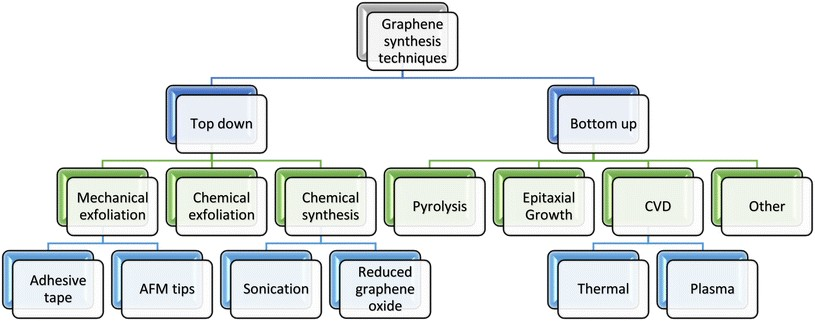
\includegraphics[width=0.9\linewidth,height=205pt]{Figures/Figure1.1.jpg} \\
  \end{tabular}
  \caption{Graphene Synthesis Process Flow Chart (Bhuyan et al., 2016)}
\end{figure}

\noindent It was discovered in 2004 that graphite could be exfoliated mechanically. A cheap and straightforward technique has widely been credited for the explosive growth in interest in graphene (Novoselov, 2004). Graphene flakes have been invaluable in elucidating graphene properties. However, they are primarily available in sizes of just a few microns, and they do not have deterministic azimuthal orientations. The flakes must be oriented in a unique azimuthal orientation on a substrate to exploit graphene’s extraordinary electronic transport properties. However, the latter structure may not be commercially relevant as the flake structure is not yet proven with flakes on a substrate (Avouris and Dimitrakopoulos, 2012). Because the scope and objectives of this report are limited, detailed graphene synthesis information cannot be reported in greater depth. A brief description of the graphene synthesis process can be provided by the flow chart shown in Figure 1.1.\vspace{\baselineskip}

\noindent The primary requirement of creating stretchable electronic devices is that the electrodes can withstand large amounts of strain ($>$1\%) without affecting electrical performance. In general, traditional electrode and interconnect materials such as single-crystal inorganic metals, polycrystalline films of evaporated metals, and metal oxides cannot be used to manufacture stretchable circuits due to their brittle nature. As a result, researchers have worked diligently on developing stretchable conductors. A general strategy consists of two main approaches. The first is to use new structural layouts on conventional electrodes. The second is developing and synthesising new materials and composites that enhance flexibility when used in special structural arrangements. Conventional electrodes can sustain sufficient conductivity in high strain while being constructed into such configurations with wavy geometries, serpentine interconnects, spiral structures, etc. Due to their ability to withstand extreme conditions involved in fabricated conductors, such as high temperatures and vacuum evaporation, they rely on costly tools. (Lee, 2020, p.175.)\vspace{\baselineskip}

\noindent The report is based on computational research as well as qualitative and quantitative research. It will be compiled using online research journals and review papers. The data analysis software and tools are mentioned in chapter 3 of the report. Although the GRANT Edu Pack software was initially intended for collection, it failed to reveal the desired data during the experiment. Enterprise software was the only one that revealed the desired data. In addition, materials derived from actual research papers can also be used to analyse the degree of reliability of the simulator model.

\subsection{Motivation}

\noindent ``The motivation for this project comes from the idea of futurism. To improve the currently used technology by investigating the use of graphene properties in various sectors of technology. The main area of focus is mobile screens. The global touchscreen market estimates at \$60.3 Billion in 2020 (Businesswire.com, 2020)" (Asif, 2020). There are currently 14.02 billion mobile devices globally, set to rise to 17.72 billion by 2024 (Statista, 2020).  Hence, there are twice as many mobile devices as there are people globally (7.8 billion), showing the touchscreen technology market is growing.\vspace{\baselineskip}

\noindent ``There are five main types of touch screens used in a phone; resistive, surface capacitive, projected capacitive, SAW (Surface Acoustic Wave), and infrared touchscreens. Capacitive touchscreens are formed from multiple layers of glass and plastic and coated with a conductor material like indium tin oxide (ITO) or copper (Cu). These conducting materials respond when contacted with an electrical conductor such as a human finger (surface capacitive) or even a surgical glove for a projected capacitive touchscreen (Sirois, 2018). These phone touchscreens' properties include image clarity, durability, resistance to surface contaminants (dust or grease), and high scratch resistance." (Asif, 2020)\vspace{\baselineskip}

\noindent The primary material used for displays, touch panels, and solar cell applications is ITO. Unfortunately, the cost per unit is increasing, and it does not have the flexibility, so the demand for new, cheaper, and more impressive material is expanding. ITO is expected to be depleted in a few years, and total mine production in the year 2020 was 900 metric tons compared to 968 metric tons in the year 2019 (Asif, 2020). The cost of crude indium increased from \$138 to \$162 per kg by the start to the end of the year (Usgs.gov, 2021).\vspace{\baselineskip}

\noindent Therefore, a replacement material must be developed with excellent mechanical and electrical properties compared with that of indium tin oxide. Graphene offers these advanced properties in conjunction with these physical qualities, such as flexibility and stretchability (Lee, 2020, p.14). “The most effective way to produce material for future touchscreens is to use nanocomposite; this is a multiphase solid material where one or more phases can have dimensions of less than 100 nm to be combined with graphene to make better overall material. The benefits include the touchscreen’s ability to be recycled; it will be lightweight and durable, so it will be hard to smash, and potentially flexible so it can fold. However, making nanocomposites for graphene is not a simple process, so this project will review the literature to understand where the field stands now. An increase in graphene usage will enable manufacturers to develop more accessible means of obtaining graphene." (Asif, 2020)

\subsection{Aims and Objectives}
\noindent This project examines the properties of graphene, particularly applying to mobile phone displays, and how it can be utilised from a manufacturing and design perspective. To be successful, graphene needs to replicate and improve upon existing manufacturing methods and procedures. The project will be executed in the following way:

\textcolor{black}{\begin{enumerate}
\item Research how graphite, graphene, graphene composites, indium tin oxide, and flexible displays have been explored scientifically and analytically.
\item Compare conventional mobile screen displays with potential graphene composite displays.
\item Simulate and model graphene composite and indium tin oxide screens with Autodesk Fusion 360 and Abaqus CAE.
\item Investigate the environmental benefits of manufacturing mobile screens using graphene.
\end{enumerate}\vspace{\baselineskip}}

\noindent To accomplish the aims above, there defined objectives are required. The following points that must be achieved:

\textcolor{black}{\begin{itemize}
\item Comparison of different parameters of graphene to other known materials, used previously or currently in the flexible display market, to determine if graphene is the most efficient and effective choice to produce flexible displays.
\item Consideration of the economic viability of graphene in future processes by looking at manufacturing costs and the amount consumers are prepared to pay for graphene-based products.
\item Establishment of results, presented graphically and by simulations, using data taken from scientific sources. Data on the composite materials will be obtained using Granta EduPack software from Ansys (CES) and academic papers and journals.
\item Use of simulation software such as Autodesk Fusion 360 to design and apply a mobile screen and then import the CAD file into Abaqus CAE to perform structural analysis on the screen. Based on the above data, graphene composites will be compared to indium tin oxide.
\end{itemize}}

\subsection{Outline for Project}

\textcolor{black}{Chapter 2 is a literature review representing up-to-date information about graphene, graphite, applications of graphene, graphene composites, and potential graphene uses in mobile phones to advance the way we use and interact with our phones.\vspace{\baselineskip}}

\noindent Chapter 3 describes how to simulate a graphene mobile screen using the finite element method. Additionally, it discusses how computation executes to simulate the screens, explaining the assumptions made. It then describes each process of analysing graphene properties, such as strength and flexibility, using the software.\vspace{\baselineskip}

\noindent Chapter 4 will present the results derived by finite element methods covering graphene and indium-tin oxide, as well as simulations and mechanical tests on strength and flexibility. These will be depicted graphically.\vspace{\baselineskip}

\noindent Chapter 5 evaluates the results obtained in the previous chapter to determine whether or not the mechanical testing was accurate, which screen was the best, the comparison between graphene and indium tin oxide simulated screens, and the limitations and improvements to the models.\vspace{\baselineskip}

\noindent Chapter 6 gives the report's overall outcome linking back to the aims and objectives of the report.\vspace{\baselineskip}

\newpage
\section{Literature Review}

\subsection{What Is Graphene?}

\noindent ``Graphene is an extraordinary material with diverse extreme properties and can be used in many applications. An existing product can be improved, or a new concept can be introduced. In Figure 2.1, graphene can be shown to have a simple atomic structure. Strong as diamond, it is also flexible like plastic. It is smaller than one-millionth of the thickness of an A4 sheet of paper. This material is extremely thin, lightweight, conductive, impermeable, and thermally conductive. (Graphenesq.com, 2014)" (Asif, 2020)\vspace{\baselineskip}

\begin{figure}[H]
  \centering
  \begin{tabular}{@{}c@{}}
    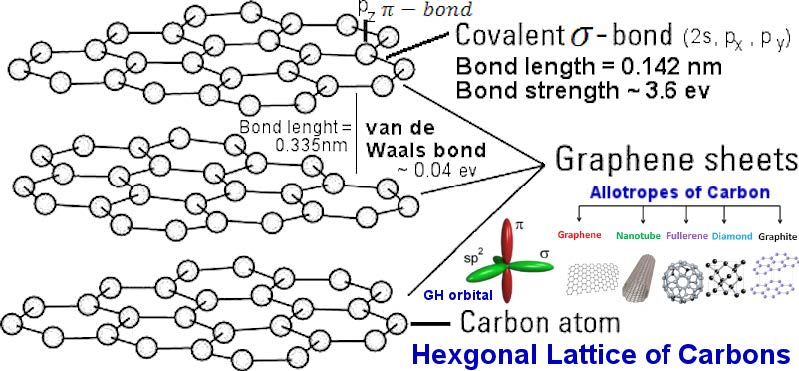
\includegraphics[width=.75\linewidth,height=200pt]{Figures/Figure2.1.jpg} \\
  \end{tabular}
  \caption{Hexagonal Lattice of Graphene (Universe-review.ca, 2018)}
\end{figure}

\noindent ``Graphene is highly transparent, with the level of optical transparency being 97.7\%, and the value of white light absorption being only 2.3\% per layer. (Sheehy and Schmalian, 2009)" (Asif, 2020)\vspace{\baselineskip}

\noindent ``Graphene is the best-known electrical conductor with an electrical resistivity of 10 $\Omega$ cm$^{-1}$, and electron mobility is limited by silicon dioxide as a substrate at around 40,000 cmV$^{-1}$s$^{-1}$. At room temperature, the value for thermal conductivity is close to 4,000 Wm$^{-1}$K$^{-1}$ (Sang et al., 2019). The most useful electrical property of graphene is its ability to act as a charge carrier for both electrons and holes. Due to their lack of mass, graphene electrons behave very similar to photons in their mobility. These charge carriers are extremely efficient at transporting information; this is known as ‘ballistic transport.’ However, there is also a constraint: its quality and substrate limit graphene production. Hence, the quality of graphene must therefore be pure or high enough to produce the phenomenon mentioned (Du et al., 2008)." (Asif, 2020)\vspace{\baselineskip}

\noindent ``One of graphene's mechanical properties is its fundamental strength; it can withstand the ultimate tensile strength of 130 GPa. Graphene is light (0.7 milligrams per square meter). It has elastic properties and can keep its original shape after strain, and this property makes it a valuable material in many fields." (Asif, 2020)

\subsection{Where Does Graphene Originate?}

\noindent ``The graphene formed from graphite. Figure 2.2 illustrates graphite, a naturally occurring form of crystalline carbon that forms in metamorphic and igneous rocks. Carbon atoms rearrange themselves into layers as they are heated to high temperatures, such as 4000 $^{o}$C to form graphite. It has many properties since it is exceptionally soft, cracks with very light pressure, and has low specific gravity. (King, H.M. 2012)." (Asif, 2020)\vspace{\baselineskip}

\begin{figure}[H]
  \centering
  \begin{tabular}{@{}c@{}}
    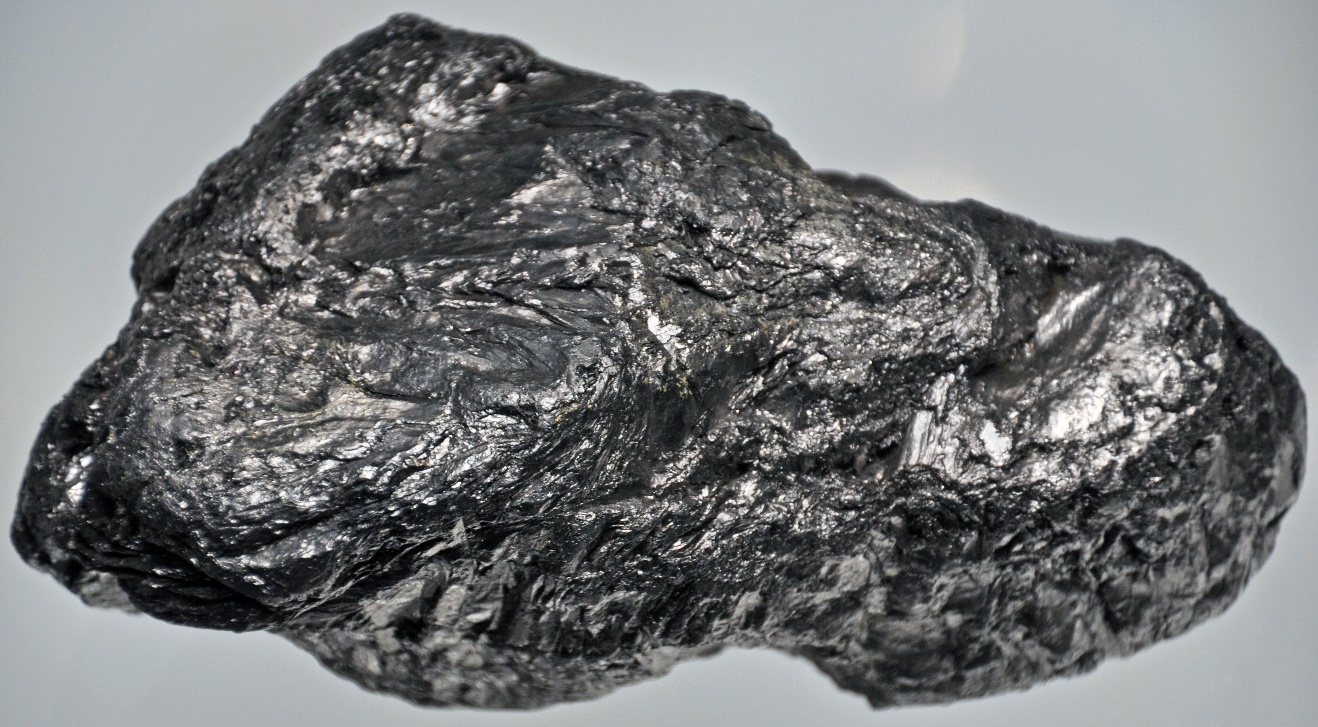
\includegraphics[width=.75\linewidth,height=200pt]{Figures/Figure2.2.jpg} \\
  \end{tabular}
  \caption{Crystalline Flake Graphite (Tirupatigraphite.com, 2017)}
\end{figure}

\noindent ``Graphene is created in numerous ways. The simplest way is to use strips of scotch tape embedded with graphite. Then split the scotch tape in half repeatedly until they form a monolayer of graphite, said to be graphene. This process can take a very long time until there is only one layer of graphite. It may be an atom-thick material, but graphene can still be seen under an optical microscope. In addition, CVD (Chemical Vapor Deposition) is known for its most significant effect on large-scale producing graphene from carbon atoms. Unfortunately, during the graphene production process, various imperfections and impurities are introduced into the graphene. Therefore, more effort will be required to reduce the production costs. (Lee, 2020, p.8)." (Asif, 2020)\vspace{\baselineskip}

\noindent ``Different graphene production processes can produce graphene with different properties; thus, manufacturers need constant feedback on the structure and quality of graphene when producing it for different applications. The producers' quality of graphene may be unacceptable, which will disrupt the search for new applications for graphene. For example, the NUS Centre for Advanced 2D Materials analysed and tested graphene samples from 60 suppliers from the Americas, Asia, and Europe. It was troubling to see that some samples were contaminated with chemical components like silicon and contained less than 10\% pure graphene flakes. (The American Ceramic Society, 2018)" (Asif, 2020)

\subsection{Applications of Graphene}

\noindent Many applications exist for graphene, such as flexible, stretchable, and foldable devices. The electrons can move freely at high speeds because of the unique arrangement of the carbon atoms in graphene. Graphene is also used in fields such as sensors, and metrology provides many advantages as every atom is exposed to the environment; thus, it is ideal for biological, gas, and chemical sensors. Among the uses of such sensors are explosive detections, selective gas sensors, and much more. (Michael Berger, 2015)

\subsection{Graphene Composites}

\noindent Graphene is well-suited to act as a reinforcing agent in composites. It can be combined with existing polymers to enhance existing materials, referred to as composite materials. Figure 2.3 below illustrates this process. It also has greater conductivity, greater robustness, greater transparency, flexibility, and so on (depending on specific needs). Additionally to lightweight composite body structures, graphene-based composite materials are used as radioactive shielding and lightning strike protection and improved fuel efficiency in aircraft (Graphene: Composite Materials, 2020). Lastly, the phone casing could be made from graphene composites since they are highly elastic, durable, and light.\vspace{\baselineskip}

\begin{figure}[H]
  \centering
  \begin{tabular}{@{}c@{}}
    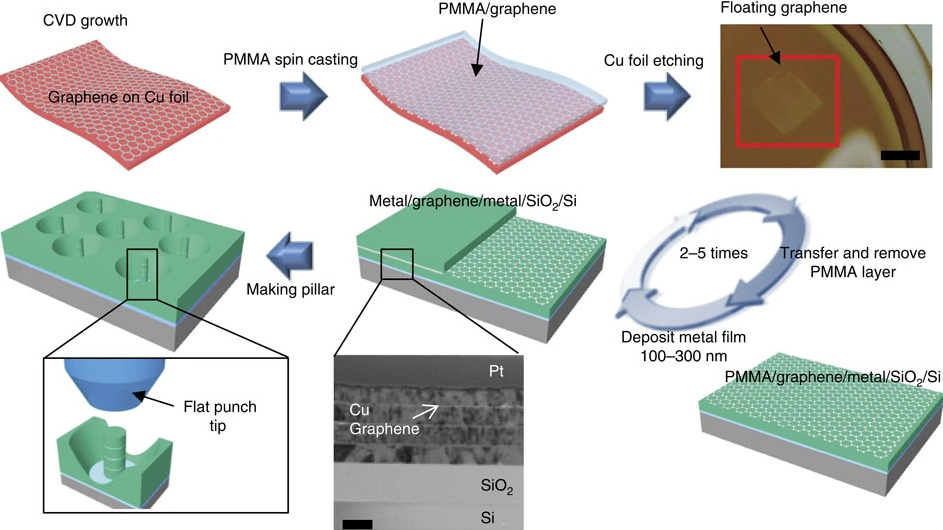
\includegraphics[width=.75\linewidth,height=200pt]{{Figures/Figure2.3.png}} \\
  \end{tabular}
  \caption{Graphene Nanolayerd Composite (Kim et al., 2013)}
\end{figure}

\subsection{Graphene for Mobile Phone Devices}

\noindent The demand for smartphones, tablets, laptops, and more has resulted in an incredible increase in touchscreen production over the years. Consequently, this will make it plausible to conclude that graphene will play an integral part in smartphone displays in the coming years. If you experiment with graphene to improve a product, it is simpler to determine whether graphene composites are suitable replacements for the product.\vspace{\baselineskip}

\noindent Displays with graphene’s flexibility, transparency and conductivity make the perfect use of graphene. Many new products utilising graphene-based conductive wires will be developed in the near future to create transparent touch panels, display backplanes, and transparent electrodes for OLEDs.\vspace{\baselineskip}

\noindent Most touchscreens currently use indium tin oxide (ITO), both transparent and conductive, but it is not easy to find and is brittle. Therefore, companies are looking to find alternatives. It would be possible to use graphene instead of ITO in displays, especially flexible displays. While graphene’s application as a flexible display does seem like a natural one and is among the first to have been commercialised (particularly in China - cqmxi.com, 2019), several other technologies seem much more advanced and more appropriate than graphene for this specific application. (Graphene-info.com, 2017)\vspace{\baselineskip}

\noindent As one of the most widely used electrodes in displays, ITO serves as a cathode in bottom-emitting displays and anode in top-emitting displays. In addition, a graphene-based cathode/anode can be used instead of an ITO-based one. (Graphene-info.com, 2017)\vspace{\baselineskip}

\noindent Display backplanes can also be made of graphene. The backplane is the driver (or electronics) used to control which pixels are turned on and off in a display. Most displays nowadays use silicon or metal TFT (thin-film transistor) substrates. Although highly conductive, graphene doesn’t have a bandgap – as such, it is unsuitable for a backplane material (Graphene-info.com, 2017). The formation of a bandgap in the electronic structure of graphene (due to chemical functionalisation such as oxidation and hydrogenation) can improve the luminous properties of LEDs. (Son et al., 2016)

\subsubsection{Conductivity} 

\noindent A particular advantage of graphene over other composite materials is its extraordinary conductivity, making it particularly suitable for touchscreen applications. When graphene is used as the conductive filler in a polymer, the conductivity becomes much higher. Most polymers have a relatively low conductivity of about 10$^{-10}$ Sm$^{-1}$, but with graphene, this conductivity can exceed 10$^{-4}$ - 10$^{-5}$ Sm$^{-1}$. (Stankovich et al., 2006)

\subsubsection{Flexibility}

\noindent Since graphene can be stretched, it can be used in stretchable electronics and displays. So far, graphene’s stretching ability has been improved and enabled to be used in stretchable electronics through structural modifications or combinations of graphene with other stretchable conducting materials. Several structural modifications or combinations make graphene more stretchable and have made it used in flexible electronics. Additionally, when structures are made flexible, attention must be paid to the bend-resistance of their components. These components must be able to resist bending without sacrificing their functionality or delamination. This can be accomplished by transferring graphene onto PET and measuring the resistance change as the bending radius increases. Researchers observed only a slight variation in the resistance of graphene when the bending radius was up to 2.3 mm (tensile strain of 6.5). If the film was bent 0.8mm (tensile strain of 18.7\%), the resistance increased initially, but it gradually returned to its original state. (Kim et al., 2009)\vspace{\baselineskip}

\noindent However, its excellent mechanical flexibility is hampered by its stiffness (340 N/m) and Young’s Modulus (0.5 TPa), which prevents its use in stretchable electronics that require stretchability above 10\%. Due to the strong bonding between carbon atoms, mechanical stress cannot be dissipated in graphene lattice. (Liu et al., 2017)

\subsubsection{Strength}

\noindent The theoretical strength of graphene is defined by its theoretical maximum strength in the absence of any defects. Having 340 Nm$^{-1}$ in-plane stiffness and 0.5 TPa Young’s Modulus, it may not be considered an ideal material for electrodes that can be stretched. Because there are no energy dissipation mechanisms for applied strain in the strong carbon-carbon network, the cracking occurs at less than 5\% strain. (Lee, 2020, p.175.)\vspace{\baselineskip}

A low-cost method must overcome mechanical limitations and sustain the extraordinary properties of graphene in stretchable, transparent devices. Theoretical calculations indicate that crumpling and interplay between different layers should reduce stiffness. When two or three graphene layers are stretched at 30\% strain, they exhibit 13 times lower resistance than single-layer graphene (Won et al., 2014). The separation energy of graphene is 0.151 - 0.45 Jm$^{-2}$ when it adheres to silicon oxide (SiO$_{2}$). By transferring graphene to PET, the separation energy dropped to 0.54 mJm$^{-1}$, suggesting that the friction between graphene and the soft polymer is smaller than that of graphene and SiO$_{2}$. Thus, the maximum strain that can be transferred to graphene when stretching the material depends on the strength of the interfacial shear between graphene and the material, which leads to a greater strain tolerance of graphene on elastomer substrates. (Lee, 2020, p.176.)

\subsubsection{Transparency}

\noindent The virtues of graphene include its flexibility and stretchability, as well as its relatively straightforward synthesis and printing processes. For transparent electrodes, graphene is particularly attractive as an alternative to the ITO during manufacturing. Monolayer graphene has a transparency of 97.7\%, compared with 90.5\% ITO (Nair et al., 2008). One study shows that a stack of four monolayers of graphene enables you to achieve a sheet resistance of 10 $\Omega$ sq$^{-1}$ with 90\% transparency (Acs.org, 2021). It is possible to refer to graphene's transparency for electronic device application as follows:\vspace{\baselineskip}

\noindent Figure 2.4 shows the UV-vis spectra with increasing numbers of graphene layers on a quartz substrate. Monolayer graphene has a 2.3\% decrease in light transmittance in the visible region, and as layer count increases, the transmittance decreases even further. (Ryu et al., 2014)\vspace{\baselineskip}

\noindent Figure 2.5 shows the UV-vis transmittance of graphene and ITO films on a PET (polyethene terephthalate) substrate. Compared to graphene-based films, ITO films are considerably opaque in short visible wavelengths and yellowish with naked eyes. (D’urso et al., 2011)\vspace{\baselineskip}

\begin{figure}[H]
  \centering
  \begin{tabular}{@{}c@{}}
    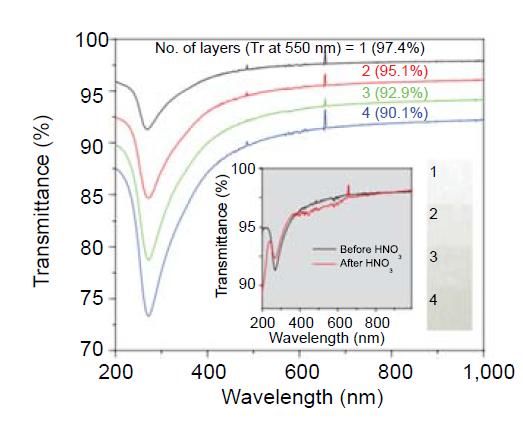
\includegraphics[width=.6\linewidth,height=200pt]{{Figures/Figure2.4.png}} \\
  \end{tabular}
  \caption{\centering Wavelength Against Transmittance of Graphene Layers on a Quartz Substrate (Lee, 2020, p.14.)}
\end{figure}

\begin{figure}[H]
  \centering
  \begin{tabular}{@{}c@{}}
    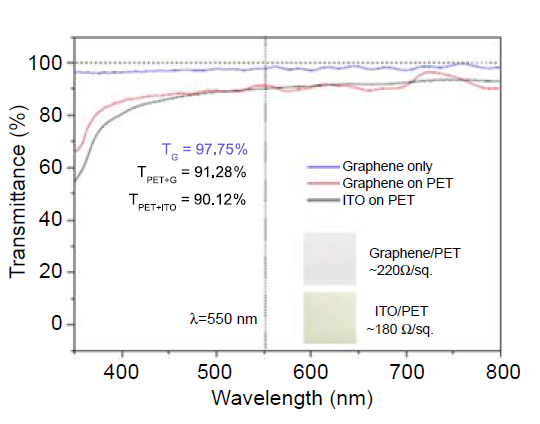
\includegraphics[width=.6\linewidth,height=200pt]{{Figures/Figure2.5.png}} \\
  \end{tabular}
  \caption{\centering Wavelength Against Transmittance of Graphene and ITO Films on a PET Substrate (Lee, 2020, p.14.)}
\end{figure}

\subsection{Commercialisation and Environmental Benefits of Graphene}

\noindent Graphene is increasingly commercialised, as highlighted by an increasing number of graphene research, patents, and applications. Graphene technologies have come a long way from laboratories to market, with applications in sports goods, automotive coatings, conductive inks, and touch screens, among others. Despite difficulties concerning quality control, advances in knowledge of graphene will drive its commercial success.\vspace{\baselineskip}

\noindent With the advent of new synthetic processes for the synthesis of graphene and its derivatives, graphene and its derivatives are now classified into two main categories: discontinuous graphene flakes of up to hundreds of micrometres and continuous graphene sheets. Both graphene types and their synthesis, properties, and products differ from one another in a significant way due to their different forms (Zhu et al., 2017). Sublimation of SiC or chemical vapour deposition (CVD) with hydrocarbon precursors can produce continuous graphene sheets (G Chiarotti and P Chiaradia, 2018). This is known as epitaxial graphene, and it is printed on the atomically flat surface of the wafer without wrinkles or contamination; it is readily able to be used in semiconductor manufacturing without the need for expensive substrates (Muñoz and Gómez-Aleixandre, 2013). This method of displays has a problem since it is chemically bonded to silicon that is not transparent. Today, the scalable graphene production process is based on the CVD process. CVD graphene suppliers are now supplying tens of meters of graphene through the roll-to-roll process. (Bae et al., 2010)\vspace{\baselineskip}

\noindent In commercial electronics, graphene electrodes have been used on mobile phone touch screens as transparent electrodes. Chongqing Graphene Technology, the company behind the flexible touch screen, describes its product as ‘Flexible wearable mobile phone, easy to carry, about 6mm ultra-thin body’, ‘Can be bent and straightened for use, cool appearance’ and ‘5.2-inch large screen mobile phone, stronger visual experience’ (Cqmxi.com, 2019). Graphene products like this are few and far between. However, there are some critical issues that need to be resolved for graphene production and standardised graphene.\vspace{\baselineskip}

\noindent In terms of graphene production, structural defects vary in length, density, and thickness based on production techniques. These defects can alter the electric or structural properties. The reduction from the outstanding graphene specifications tends to lead to failures in products with current specifications and prevents applications whose intrinsic properties are critical to creating the material. (Kong et al., 2019)\vspace{\baselineskip}

\noindent It is one of the fundamental problems in graphene production due to the run-to-run variation in graphene quality, defects, thickness, doping, etc. (Kauling et al., 2018). Different manufacturers sell graphene with a vastly different set of properties. A recent study has determined that most of the products from these manufacturers are unsuitable for most graphene applications. These manufacturers sell graphene at ridiculously high prices but do not have any minimum standards, so it is detrimental to graphene's commercialisation.\vspace{\baselineskip}

\noindent It is necessary to have publishing standards for graphene in academia in order for the standards to improve. Quality control factors include uniformity of thickness, macroscopic defects such as tears and wrinkles, and microscopically deficient features such as grain boundaries or contamination. The Raman Spectroscopy method is widely used to characterise graphene methods, but it is not effective in detecting large areas. Thus, different techniques are being used to detect the quality of graphene, which includes optical microscopy and interference reflection microscopy to visualise any cracks, voids, wrinkles, and the number of layers of graphene applied to the transparent substrate. The number of graphene-testing techniques which have been developed is increasing. This would allow a further increase in graphene commercialisation if more industries engage in it, provided graphene can process and succeed in scalable commercial applications. (Kong et al., 2019)

\newpage
\section{Using FEM to Simulate Graphene Mobile Screens}

\subsection{What is FEM?}

\noindent Finite element method (FEM) is a mathematical technique used to analyse any given physical phenomenon through finite element analysis (FEA). In places where experimental analysis is unaffordable, it is widely used for solving problems in traditional fields of engineering and nanotechnology. This numerical technique provides accurate solutions to complex engineering problems.

\subsection{Using FEM to Analyse the Mobile Screen}

\noindent A first step towards analysing mobile screens is to make a 3D model of the screen, which can be subdivided into parts, which will help to make the model accurate. This requires a considerable amount of processing power and can be difficult if most of the material properties of a part are not available or the schematic model of the 3D structure. I made an active decision to make a single object and analyse the composite as a whole since it is easier to get information about the material properties for the overall composite.\vspace{\baselineskip}

\noindent The following parameters relate to material mechanical properties for FEM analysis. 

\begin{itemize}
\item Young’s Modulus is the measure of the stiffness of an elastic material; it is defined as the ratio of stress and strain. (Ma, Sobernheim and Garzon, 2016)
\item Poisson’s ratio is the ratio of transverse strain to the corresponding axial strain applied to a stressed material along one axis. (Zhang, 2019)
\item Stress is simply a ratio of the external forces to the cross-sectional area of the material. It is measured according to what the material feels from externally applied forces. (Bu.edu, 2021)
\item Strain describes deformations attributable to stress, whether resulting from pressure or friction. It is a ratio of the change in length divided by the original length. (Bu.edu, 2021)
\item Von Mises Stress enables the determination of whether a material will yield or fracture. (SimScale, 2021)
\end{itemize}

\subsection{What Tests Will Be Performed on the Mobile Screens?}

\subsubsection{Analysing the Flexibility of the Mobile Screens}

\noindent The flexibility of the mobile screens can also be calculated using FEM by bending the screens at different angles. Half of the screen will be fixed, and on the opposite side, there will be a displacement boundary condition, in which the angle will be perpendicular to the mobile screen. The displacement angle could be determined by using the trigonometric formula below:

\begin{equation}
I = \frac{L sin(\theta)}{2}
\end{equation}

\noindent where:\newline
I - Imposed Displacement (mm)\newline
L - Length of the Screen (mm)\newline
$\theta$ - Bending Angle (degrees)

\begin{figure}[H]
  \centering
  \begin{tabular}{@{}c@{}}
    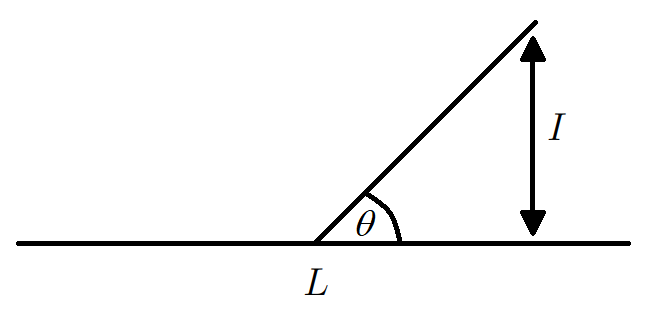
\includegraphics[width=.75\linewidth,height=200pt]{{Figures/Figure3.1.png}} \\
  \end{tabular}
  \caption{Schematic of Imposed Displacement Calculation of the Mobile Screen}
\end{figure}

\noindent Abaqus will compute stresses and strains on the simulated screen based on information concerning imposed displacement, utilising the method described in figure 3.1, then determine maximum areas of imposed displacements and stresses at the bend angles about which comparisons can be made with that of different materials.

\subsubsection{Analysing the Strength of the Mobile Screens}

\noindent The strength of mobile screens can be measured with the application of point loads. Different loads can be applied to the centre of screens, while the edges of the screens remain fixed, determined by boundary conditions. After the material has been stressed to the maximum, FEM can show the maximum deformation and stresses due to the increasing load. This can be used to compare other materials and see which material performed the best. Essentially, what matters is the strength of the material. Will it fail or not, and if it does, then it will have reached its failure region, or else it is outside the elastic limit. Figure below shows how the screen would be tested using FEM in Abaqus CAE.

\begin{figure}[H]
  \centering
  \begin{tabular}{@{}c@{}}
    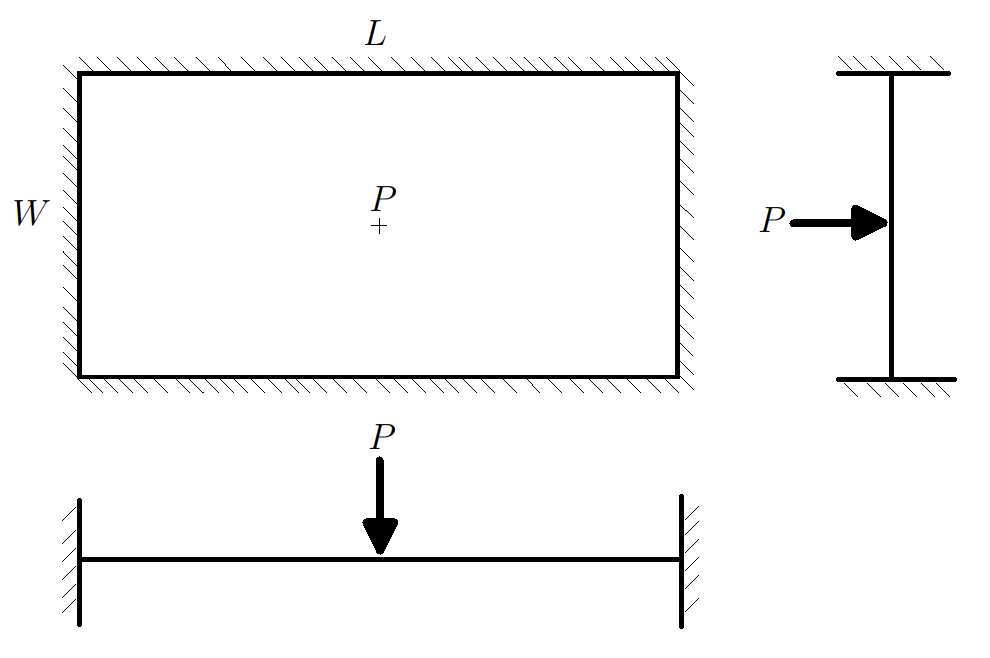
\includegraphics[width=.75\linewidth,height=200pt]{{Figures/Figure3.2.png}} \\
  \end{tabular}
  \caption{Schematic of Point Loading on the Mobile Screen}
\end{figure}

\noindent where:\newline
P - Represents the Load (N)\newline
L - Length of the Screen (mm)\newline
W - Width of the Screen (mm)

\newpage
\subsection{Computational Procedure}

\noindent Simulating a screen requires some primary conditions to be considered. So, for each simulation, the material's mechanical properties, dimensions, and boundary conditions must be explicitly specified numerically. Table 3 gives characteristics of six different materials.\vspace{\baselineskip}

\noindent \textbf{Dimensions:} The first step of the part model is to create a sketch using iPhone 11 Pro Max as a reference phone, then the screen is modelled with 165.1mm height, 76.7mm width, and extruded to 0.3mm thickness. (Device Specifications, 2012)\vspace{\baselineskip}

\begin{figure}[H]
  \centering
  \begin{tabular}{@{}c@{}}
    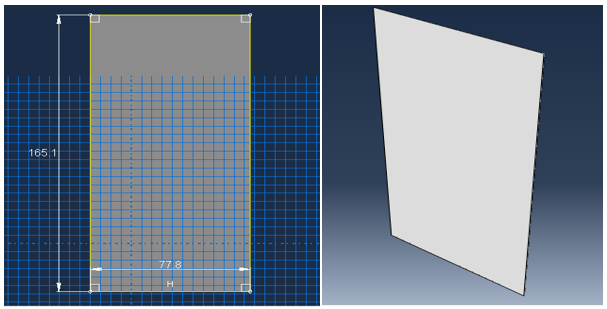
\includegraphics[width=.75\linewidth,height=230pt]{{Figures/Figure3.3.png}} \\
  \end{tabular}
  \caption {Sketch (left) and Extruded Part Model (right) in Abaqus CAE}
\end{figure}

\noindent To create a material with the properties specified in Table 3, choose the property’s module, then by choosing Material $>$ Create on the main menu bar, choose Mechanical $>$ Elasticity $>$ Elastic. In this way, 6 properties can be assigned to all 6 screens.

\begin{figure}[H]
  \centering
  \begin{tabular}{@{}c@{}}
    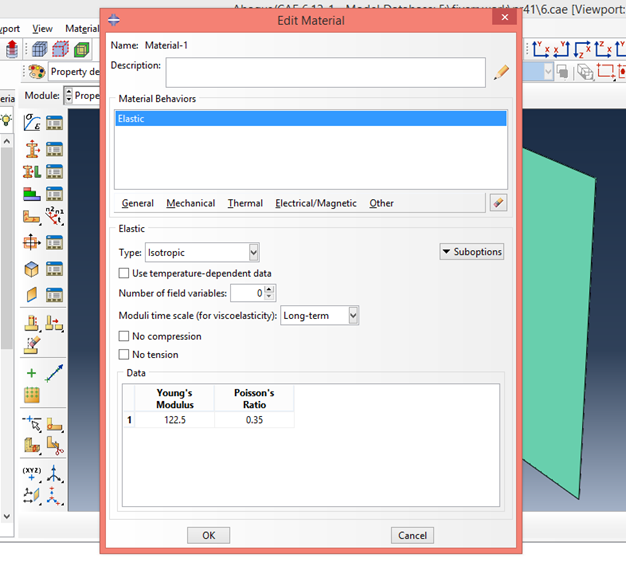
\includegraphics[width=.75\linewidth,height=260pt]{{Figures/Figure3.4.png}} \\
  \end{tabular}
  \caption {Creating a Material in Abaqus CAE}
\end{figure}

\noindent Once the material has been created, it is necessary to define a section to be assigned to a part. A solid homogeneous section is defined here that best represents the model properties, and then it is assigned to the screen.\vspace{\baselineskip}

\begin{figure}[H]
  \centering
  \begin{tabular}{@{}c@{}}
    \includegraphics[width=.75\linewidth,height=240pt]{{Figures/Figure3.5.png}} \\
  \end{tabular}
  \caption {Creating a Material Section in Abaqus CAE}
\end{figure}

\noindent \textbf{Assembly:} The screen can be assembled using an independent instance, which allows the screen to mesh and provides capabilities such as adding partitions and creating virtual topologies. The downsides of independent instances include the fact that they consume more memory and be meshed individually. To do this, click the assembly module, then select Instance $>$ Create.\vspace{\baselineskip}

\begin{figure}[H]
  \centering
  \begin{tabular}{@{}c@{}}
    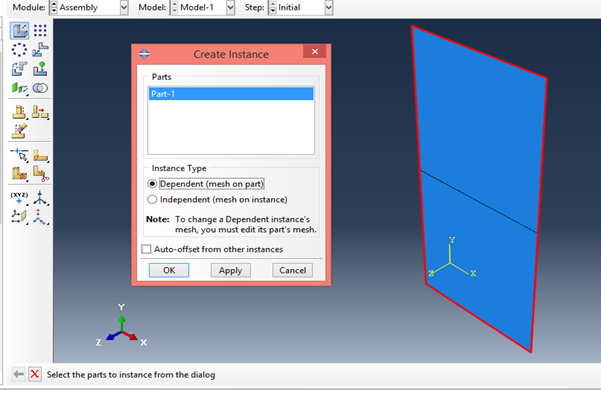
\includegraphics[width=.75\linewidth,height=230pt]{{Figures/Figure3.6.png}} \\
  \end{tabular}
  \caption {Creating an Assembly Instance in Abaqus CAE}
\end{figure}

\noindent \textbf{Step:} Detailed static analysis is performed both in a bending application and a point loading application. This can be done by selecting step module, then Step $>$ Create, and choosing Static, General.\vspace{\baselineskip}

\begin{figure}[H]
  \centering
  \begin{tabular}{@{}c@{}}
    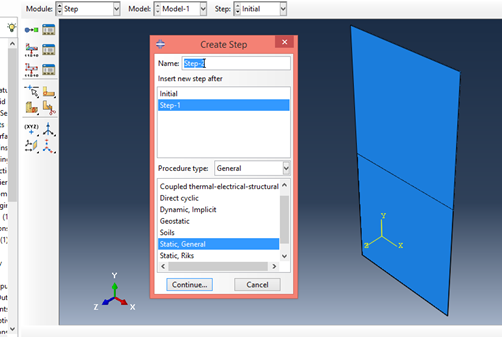
\includegraphics[width=.75\linewidth,height=230pt]{{Figures/Figure3.7.png}} \\
  \end{tabular}
  \caption {Creating Step for Static Analysis in Abaqus CAE}
\end{figure}

\noindent \textbf{Boundary and Loading Condition:} To experiment with load variations, 5 different loading factors are applied at the centre of the screen. Selecting load module then, Load $>$ Boundary Condition. The magnitude of the load applied for each case is shown in Table 1.\vspace{\baselineskip}

\begin{figure}[H]
  \centering
  \begin{tabular}{@{}c@{}}
    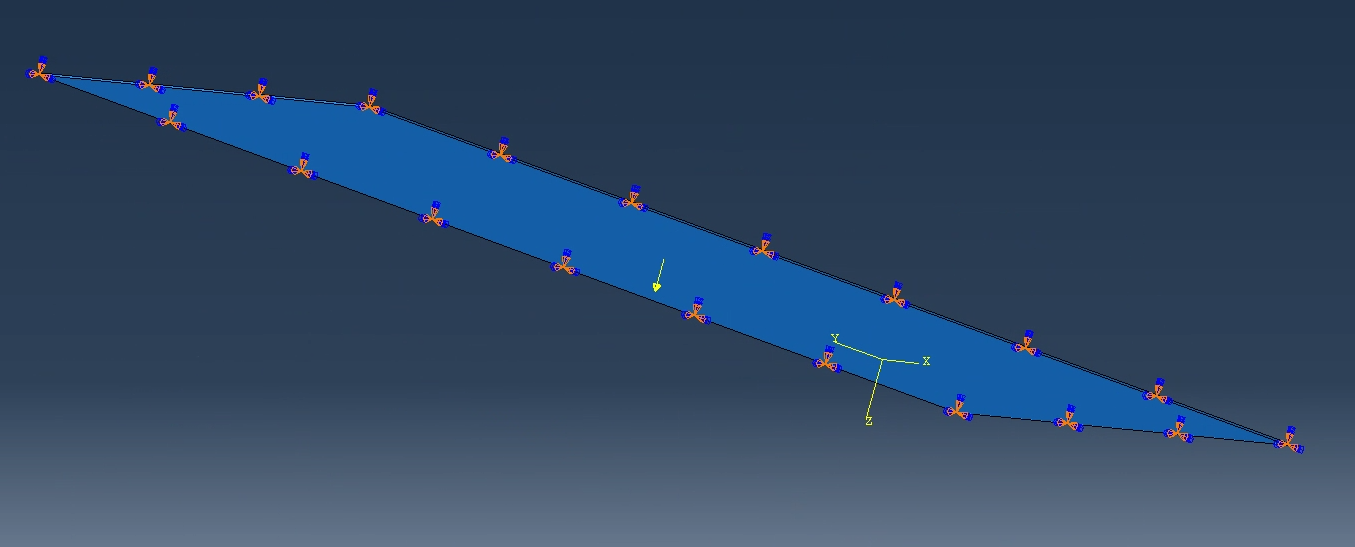
\includegraphics[width=.75\linewidth,height=235pt]{{Figures/Figure3.8.png}} \\
  \end{tabular}
  \caption {Illustration of Boundary Conditions for Point Loading Set on Abaqus CAE}
\end{figure}

\noindent For bending a screen, half of the screen is fixed, and on the other side, a boundary condition based on a displacement is provided such that the screen may be bent at the required angle. The magnitude of each angle is adjusted separately, as it is with every point load. Table 2 below gives the imposed displacements at each angle.\vspace{\baselineskip}

\begin{figure}[H]
  \centering
  \begin{tabular}{@{}c@{}}
    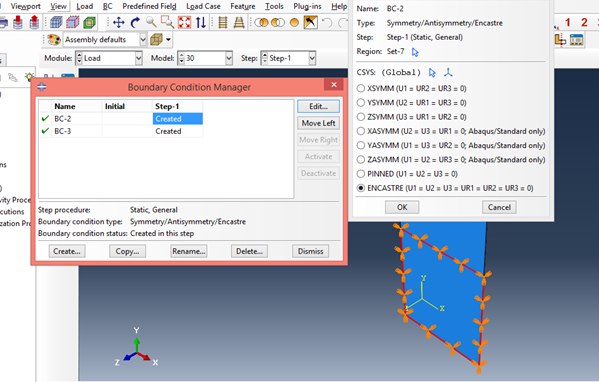
\includegraphics[width=.75\linewidth,height=230pt]{{Figures/Figure3.9.png}} \\
  \end{tabular}
  \caption {Illustration of Boundary Conditions for Bending Case Set in Abaqus CAE}
\end{figure}

\begin{figure}[H]
  \centering
  \begin{tabular}{@{}c@{}}
    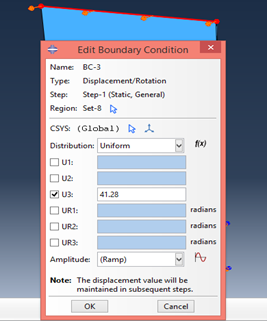
\includegraphics[width=.45\linewidth,height=230pt]{{Figures/Figure3.10.png}} \\
  \end{tabular}
  \caption {Imposed Angle Boundary Condition for Bending Case Set in Abaqus CAE}
\end{figure}

\FloatBarrier
\begin{table}[hbt!]
\centering
\caption{Point Loading Data}
\begin{tabular}{|c|c|}
\hline
\textbf{Type of Loading} & \textbf{Magnitude of Loading (N)} \\ \hline
Load 1                   & 5                                 \\ \hline
Load 2                   & 10                                \\ \hline
Load 3                   & 15                                \\ \hline
Load 4                   & 20                                \\ \hline
Load 5                   & 25                                \\ \hline
\end{tabular}
\end{table}

\begin{table}[hbt!]
\centering
\caption{Bending Angle Data}
\begin{tabular}{|c|c|}
\hline
\textbf{Bending Angle} & \textbf{Imposed Displacement (mm)} \\ \hline
15$^{\circ}$           & 21.37                              \\ \hline
30$^{\circ}$           & 41.28                              \\ \hline
45$^{\circ}$           & 58.37                              \\ \hline
60$^{\circ}$           & 71.49                              \\ \hline
90$^{\circ}$           & 82.55                              \\ \hline
\end{tabular}
\end{table}
\FloatBarrier

\noindent \textbf{Mesh:} The model is meshed with C3D8R elements, which are 8-node linear bricks, reduced integration, hourglass control. In general, this element type is used because it produces accurate results for this kind of analysis, and it is the default when meshing the screen.\vspace{\baselineskip}

\begin{figure}[H]
  \centering
  \begin{tabular}{@{}c@{}}
    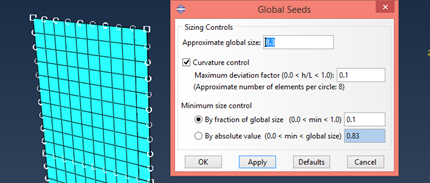
\includegraphics[width=.7\linewidth,height=182pt]{{Figures/Figure3.11.png}} \\
  \end{tabular}
  \caption {Mesh Element Size Set in Abaqus CAE}
\end{figure}

\noindent \textbf{Job:} In Figures 3.12 and 3.13 below shows the job manager. A new job can be created, and the status of it can be monitored. Post-processing job results can be viewed here once they are complete.\vspace{\baselineskip}

\begin{figure}[H]
  \centering
  \begin{tabular}{@{}c@{}}
    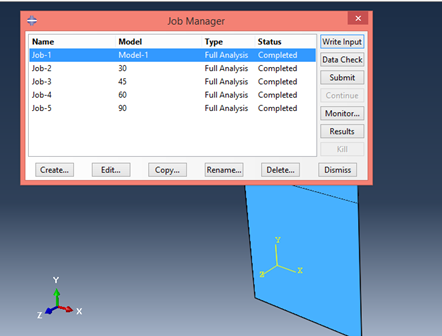
\includegraphics[width=.75\linewidth,height=230pt]{{Figures/Figure3.12.png}} \\
  \end{tabular}
  \caption {Job Manager in Abaqus CAE}
\end{figure}

\begin{figure}[H]
  \centering
  \begin{tabular}{@{}c@{}}
    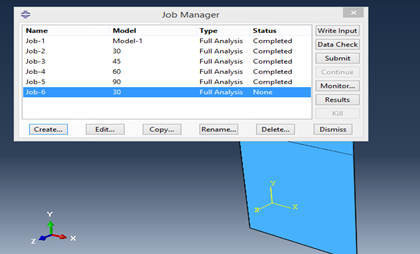
\includegraphics[width=.75\linewidth,height=230pt]{{Figures/Figure3.13.png}} \\
  \end{tabular}
  \caption {Creating New Job in Abaqus CAE}
\end{figure}

\noindent \textbf{Visualisation:} When the job status progresses to completed, required results are displayed as ’S’ representing Von Mises stress results and ’U’ representing displacement results.\vspace{\baselineskip}

\begin{figure}[H]
  \centering
  \begin{tabular}{@{}c@{}}
    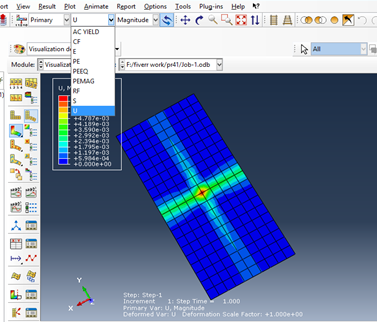
\includegraphics[width=.75\linewidth,height=240pt]{{Figures/Figure3.14.png}} \\
  \end{tabular}
  \caption {Visualisation of Displacement in Abaqus CAE}
\end{figure}

\begin{figure}[H]
  \centering
  \begin{tabular}{@{}c@{}}
    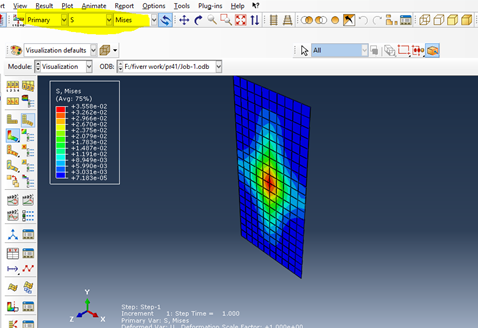
\includegraphics[width=.75\linewidth,height=240pt]{{Figures/Figure3.15.png}} \\
  \end{tabular}
  \caption {Visualisation of Von Mises Stress in Abaqus CAE}
\end{figure}

\newpage
\section{Results}

\subsection{Initial Parameters}


\begin{table}[hbt!]
\caption{Materials Properties}
\resizebox{\textwidth}{!}{%
\begin{tabular}{|c|l|c|c|}
\hline
\textbf{Material No.} & \multicolumn{1}{c|}{\textbf{Material}}                  & \textbf{\boldmath{$E$} (MPa)} & \textbf{\boldmath$\upsilon$} \\ \hline
Material 1 & Graphene loading wt 0.6\% (Hameed et al., 2018)            & 650    & 0.3  \\ \hline
Material 2 & Graphene content 10-TOCN-RGO (Zhan et al., 2019)           & 8400   & 0.3  \\ \hline
Material 3 & Bioinspired films PGA/GO/Ca2+ (Liang et al., 2020)          & 1700   & 0.3  \\ \hline
Material 4 & Graphene Reinforced Epoxy Nanocomposites EEG 0.05vol.\% (Xin Zhao, 2017) & 2520 & 0.3 \\ \hline
Material 5 & Graphene Nanocomposites (0.1\% wt GPL) (Rafiee et al., 2009) & 3750   & 0.3  \\ \hline
Material 6 & Indium Tin Oxide (Lee et al., 2011) & 117500 & 0.35 \\ \hline
\end{tabular}%
}
\end{table}

\noindent Material 1 was chosen because it was the first to employ epoxy thermosets. Its flexibility was achieved by adding charge transfer complexes that involved functional groups within cross-linked epoxy and ions from room temperature ionic liquids. There was a constant increase in the mechanical properties of epoxy with the addition of 0.6 wt\% graphene. A 0.6\% addition increased the tensile strength by 125\% and Young's Modulus by 21\%. In the nanocomposites, electrical resistance increased with graphene loading, which indicates that phase separation occurs between the ionic liquids and graphene sheets in the matrix. It behaved just like a ductile thermoplastic when exposed at room temperature. (Hameed et al., 2018)\vspace{\baselineskip}

\noindent Cellulose nanofibrils made from wood are natural polymer nanomaterials with high specific surface areas, low density, high strength, and high modulus of elastic deformation. To prepare conductive nanocomposite films, pristine graphene (PG) was exfoliated with triethanolamine, and TEMPO-oxidised cellulose nanofibrils (TOCN) were added to it. To demonstrate their compatibility with TOCN, graphene oxide (GO) and reduced graphene oxide (RGO) have also been composited. Although Material 2 (TOCN) didn't perform as well as expected during the experiment, it was favoured since it exhibited some comparable performance and used the chemical exfoliation method shown in figure 1.1. TOCN-RGO composite films with high conductivity are essential in developing and producing low-cost, flexible metal-based electronics. (Zhan et al., 2019)\vspace{\baselineskip}

\noindent Material 3 was chosen because it is influenced by the relationship between organic and inorganic components within the hierarchical structure of nacre found in mollusc shells. It enables the fabrication of self-assembled, layered composite films made from graphene. This composite is predominantly made from polyglutamic acid produced by bacteria. It is an environmentally friendly and economic process which was the main reason it was chosen. GO, PGA, and divalent cations (Ca$^{2+}$) were used in a slow solvent evaporation process at ambient temperature to form nacre-like layered structures. Nanocomposite films made of biobased materials showed impressive mechanical properties, resulting from synergistic hydrogen bonding with the PGA and ionic bonding with calcium ions. In the composite films, the strength and Young’s Modulus are improved by about 12\% and over 70\% compared with pure GO films. (Liang et al., 2020)\vspace{\baselineskip}

\noindent Material 4 EEG (Electrochemical exfoliated graphene) 0.05 vol.\% was prepared by electrochemically exfoliating graphite into graphene in a liquid solution of inorganic salts. It was a unique process, and that is why material 4 was chosen. The electrochemical system is made of stainless-steel cathode and graphite foil anode. The electrolyte is an ammonium sulphate water solution with a concentration of 0.1 M. All other materials were sourced from other companies. In contrast, EEG was one of the materials prepared in the lab. (Xin Zhao, 2017)\vspace{\baselineskip}

\noindent Material 5 was chosen because the results in the report indicate graphene platelets perform significantly better than carbon nanotube additives. A nanofiller weight fraction of ${0.1}\pm{0.002\%}$ was used to compare the mechanical properties of epoxy nanocomposites with graphene platelets, single-walled carbon nanotubes, and multi-walled carbon nanotubes. In a sulphuric-nitric-potassium chlorate solution for 96 hours, graphite oxide was produced by oxidising it. Graphite oxide powder (200 mg) was placed in a 200 mm inner diameter, one m long quartz tube with a seal at one end to exfoliate by thermal exfoliation. An argon inlet was then inserted through the rubber stopper on the other end of the quartz tube. It was flushed for 10 minutes on argon, then fastened into the tube furnace, set to 1050 °C, and held for 30s. (Rafiee et al., 2009)
\vspace{\baselineskip}

\noindent Material 6, which is ITO, was selected to compare the values with other graphene nanocomposite materials already chosen above. In the report, a thermomechanical analyser (TMA) was used to analyse thermal strain on PET substrates and PET-ITO substrates at applied temperatures. Although the ITO layer on PET-ITO substrate has a lower coefficient of thermal expansion (CTE) and higher elastic modulus, it was observed that the thermal strain of PET-ITO substrate was related to that of PET. From these results, it was expected that the modified PET with improved thermal stability would be applied to PET-ITO as a mass production substrate. This means that ITO can therefore be used against graphene nanocomposites to see how they compare. (Lee et al., 2011)

\subsection{Simulation of Graphene Screens}

\noindent In this section, visualisations providing the stresses and displacements induced by point loading and bending of the screens using material 1 properties and their respective magnitude are provided. The resulting data for all other materials are provided in the appendix.\vspace{\baselineskip}

\newpage
\noindent Material 1 - Point Loading 
\begin{figure}[H]
  \centering
  \begin{tabular}{@{}c@{}}
    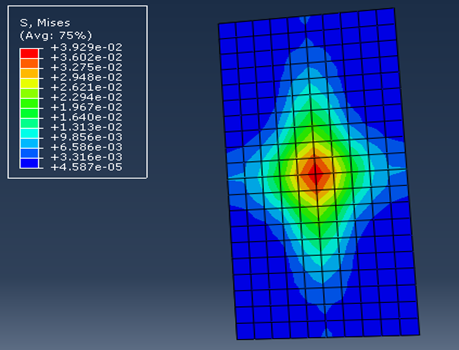
\includegraphics[width=0.7\linewidth,height=255pt]{Results/Point Loading/M1_VMS_L1.png} \\
  \end{tabular}
  \caption{Von Mises Stress (MPa) - Material 1, Load: 5N}
\end{figure}

\begin{figure}[H]
  \centering
  \begin{tabular}{@{}c@{}}
    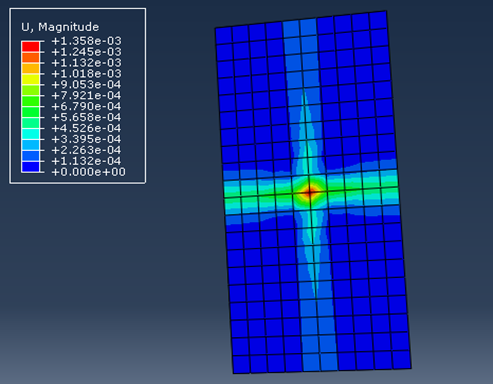
\includegraphics[width=0.7\linewidth,height=255pt]{Results/Point Loading/M1_DIS_L1.png} \\
  \end{tabular}
  \caption{Displacement (mm) - Material 1, Load: 5N}
\end{figure}

\begin{figure}[H]
  \centering
  \begin{tabular}{@{}c@{}}
    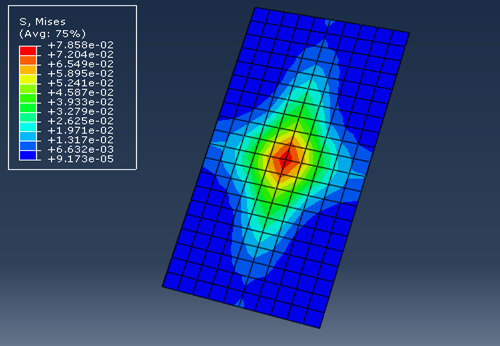
\includegraphics[width=0.7\linewidth,height=255pt]{Results/Point Loading/M1_VMS_L2.png} \\
  \end{tabular}
  \caption{Von Mises Stress (MPa) - Material 1, Load: 10N}
\end{figure}

\begin{figure}[H]
  \centering
  \begin{tabular}{@{}c@{}}
    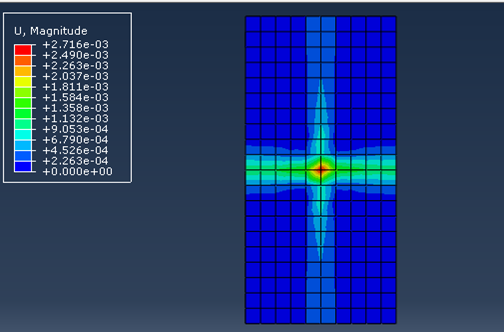
\includegraphics[width=0.7\linewidth,height=255pt]{Results/Point Loading/M1_DIS_L2.png} \\
  \end{tabular}
  \caption{Displacement (mm) - Material 1, Load: 10N}
\end{figure}

\begin{figure}[H]
  \centering
  \begin{tabular}{@{}c@{}}
    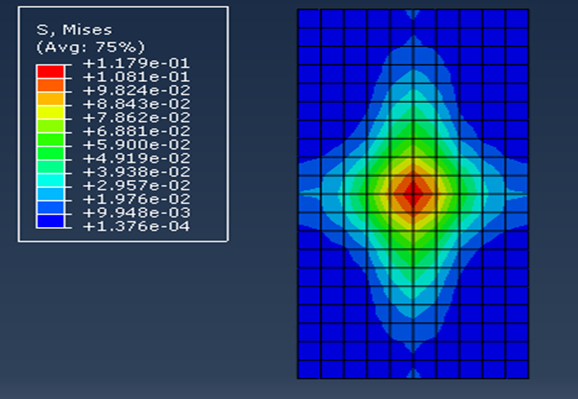
\includegraphics[width=0.7\linewidth,height=255pt]{Results/Point Loading/M1_VMS_L3.png} \\
  \end{tabular}
  \caption{Von Mises Stress (MPa) - Material 1, Load: 15N}
\end{figure}

\begin{figure}[H]
  \centering
  \begin{tabular}{@{}c@{}}
    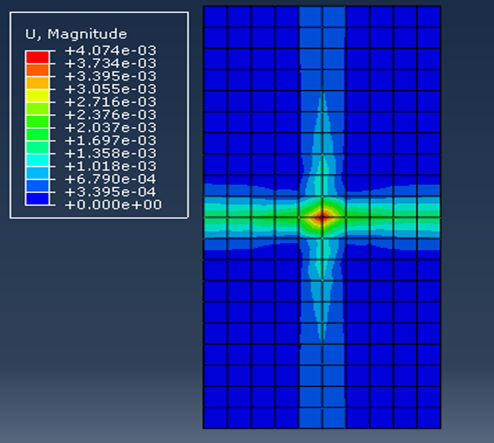
\includegraphics[width=0.7\linewidth,height=255pt]{Results/Point Loading/M1_DIS_L3.png} \\
  \end{tabular}
  \caption{Displacement (mm) - Material 1, Load: 15N}
\end{figure}

\begin{figure}[H]
  \centering
  \begin{tabular}{@{}c@{}}
    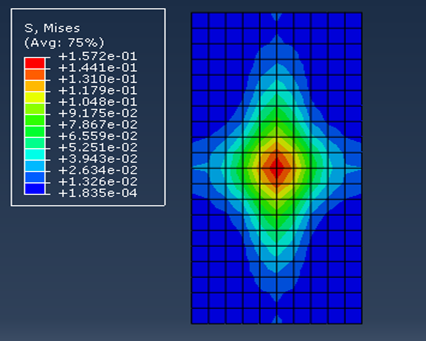
\includegraphics[width=0.7\linewidth,height=255pt]{Results/Point Loading/M1_VMS_L4.png} \\
  \end{tabular}
  \caption{Von Mises Stress (MPa) - Material 1, Load: 20N}
\end{figure}

\begin{figure}[H]
  \centering
  \begin{tabular}{@{}c@{}}
    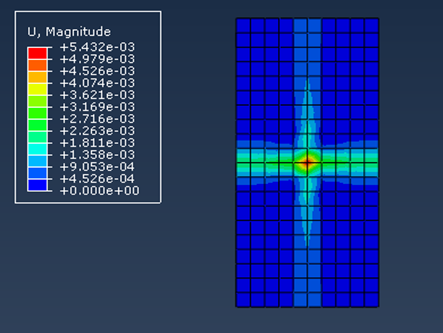
\includegraphics[width=0.7\linewidth,height=255pt]{Results/Point Loading/M1_DIS_L4.png} \\
  \end{tabular}
  \caption{Displacement (mm) - Material 1, Load: 20N}
\end{figure}

\begin{figure}[H]
  \centering
  \begin{tabular}{@{}c@{}}
    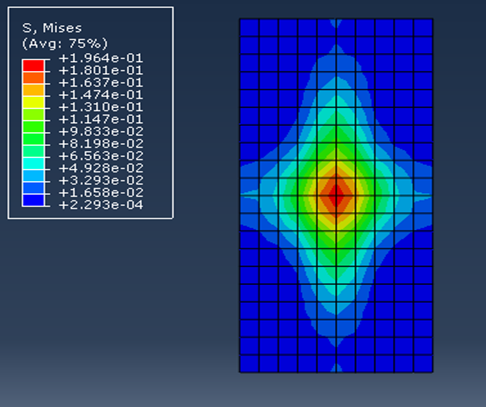
\includegraphics[width=0.7\linewidth,height=255pt]{Results/Point Loading/M1_VMS_L5.png} \\
  \end{tabular}
  \caption{Von Mises Stress (MPa) - Material 1, Load: 25N}
\end{figure}

\begin{figure}[H]
  \centering
  \begin{tabular}{@{}c@{}}
    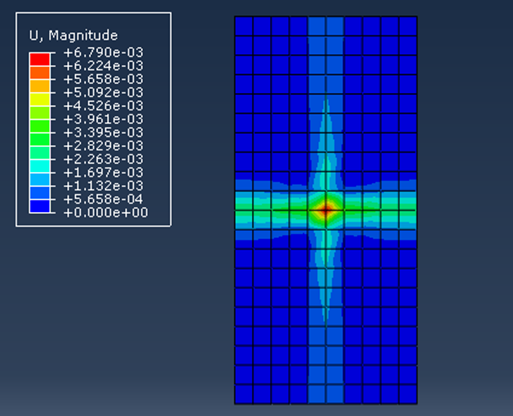
\includegraphics[width=0.7\linewidth,height=255pt]{Results/Point Loading/M1_DIS_L5.png} \\
  \end{tabular}
  \caption{Displacement (mm) - Material 1, Load: 25N}
\end{figure}

%--------------------------------------------------------------------------------------------------

\newpage
\noindent Material 1 - Bending Analysis 
\begin{figure}[H]
  \centering
  \begin{tabular}{@{}c@{}}
    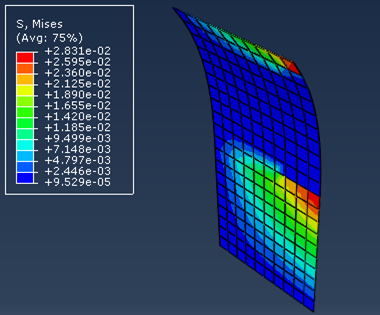
\includegraphics[width=0.7\linewidth,height=255pt]{Results/Bending/M1_VMS_15.png} \\
  \end{tabular}
  \caption{Von Mises Stress (MPa) - Material 1,  Bending Angle: 15$^{\circ}$ }
\end{figure}

\begin{figure}[H]
  \centering
  \begin{tabular}{@{}c@{}}
    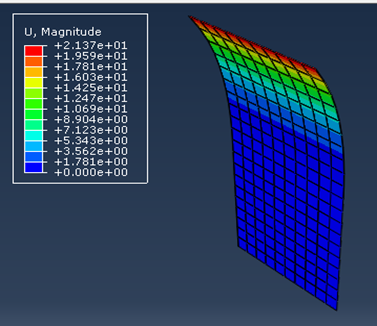
\includegraphics[width=0.7\linewidth,height=255pt]{Results/Bending/M1_DIS_15.png} \\
  \end{tabular}
  \caption{Displacement (mm) - Material 1,  Bending Angle: 15$^{\circ}$ }
\end{figure}

\begin{figure}[H]
  \centering
  \begin{tabular}{@{}c@{}}
    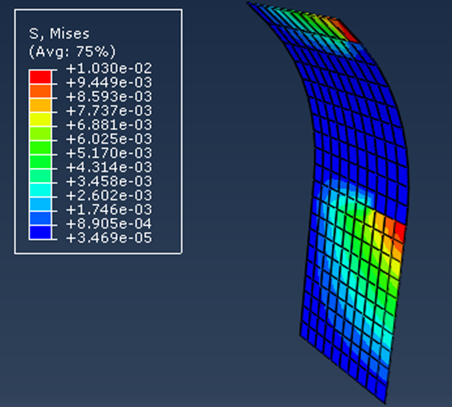
\includegraphics[width=0.7\linewidth,height=255pt]{Results/Bending/M1_VMS_30.png} \\
  \end{tabular}
  \caption{Von Mises Stress (MPa) - Material 1,  Bending Angle: 30$^{\circ}$ }
\end{figure}

\begin{figure}[H]
  \centering
  \begin{tabular}{@{}c@{}}
    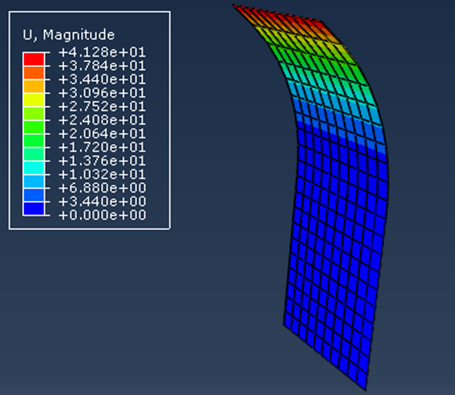
\includegraphics[width=0.7\linewidth,height=255pt]{Results/Bending/M1_DIS_30.png} \\
  \end{tabular}
  \caption{Displacement (mm) - Material 1, Bending Angle: 30$^{\circ}$ }
\end{figure}

\begin{figure}[H]
  \centering
  \begin{tabular}{@{}c@{}}
    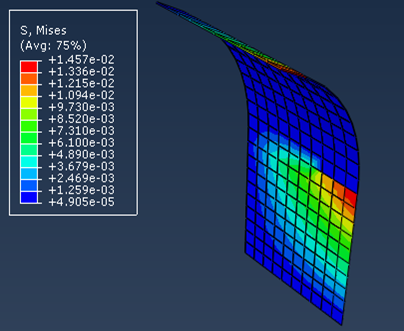
\includegraphics[width=0.7\linewidth,height=255pt]{Results/Bending/M1_VMS_45.png} \\
  \end{tabular}
  \caption{Von Mises Stress (MPa) - Material 1,  Bending Angle: 45$^{\circ}$ }
\end{figure}

\begin{figure}[H]
  \centering
  \begin{tabular}{@{}c@{}}
    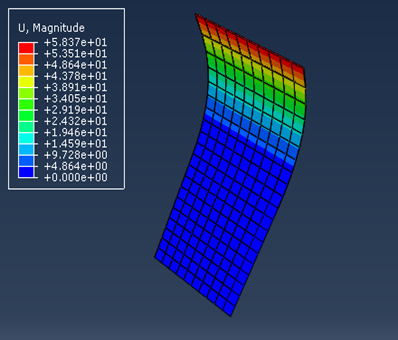
\includegraphics[width=0.7\linewidth,height=255pt]{Results/Bending/M1_DIS_45.png} \\
  \end{tabular}
  \caption{Displacement (mm) - Material 1, Bending Angle: 45$^{\circ}$ }
\end{figure}

\begin{figure}[H]
  \centering
  \begin{tabular}{@{}c@{}}
    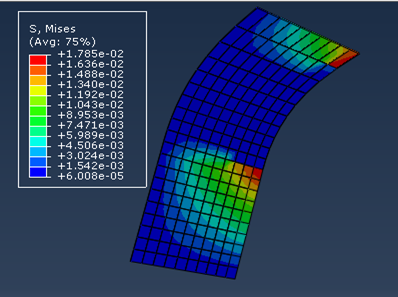
\includegraphics[width=0.7\linewidth,height=255pt]{Results/Bending/M1_VMS_60.png} \\
  \end{tabular}
  \caption{Von Mises Stress (MPa) - Material 1,  Bending Angle: 60$^{\circ}$ }
\end{figure}

\begin{figure}[H]
  \centering
  \begin{tabular}{@{}c@{}}
    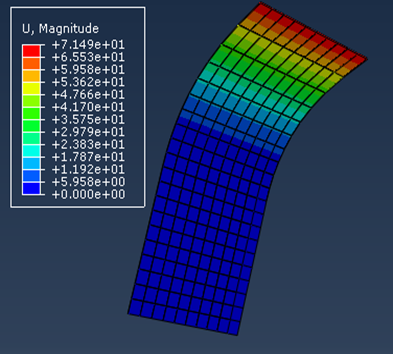
\includegraphics[width=0.7\linewidth,height=255pt]{Results/Bending/M1_DIS_60.png} \\
  \end{tabular}
  \caption{Displacement (mm) - Material 1, Bending Angle: 60}
\end{figure}

\begin{figure}[H]
  \centering
  \begin{tabular}{@{}c@{}}
    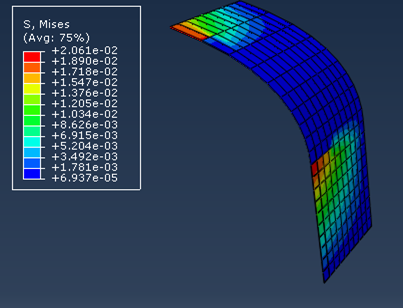
\includegraphics[width=0.7\linewidth,height=255pt]{Results/Bending/M1_VMS_90.png} \\
  \end{tabular}
  \caption{Von Mises Stress (MPa) - Material 1,  Bending Angle: 90$^{\circ}$ }
\end{figure}

\begin{figure}[H]
  \centering
  \begin{tabular}{@{}c@{}}
    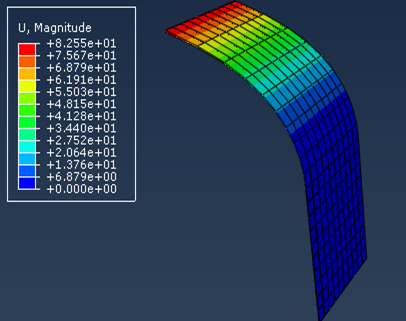
\includegraphics[width=0.7\linewidth,height=255pt]{Results/Bending/M1_DIS_90.png} \\
  \end{tabular}
  \caption{Displacement (mm) - Material 1, Bending Angle: 90$^{\circ}$ }
\end{figure}

\subsection{Simulation of Indium Tin Oxide Screen}

\noindent The visuals below illustrate the stresses and displacements (the respective magnitudes) on screens under point loading and bending analyses with material 6 properties. \vspace{\baselineskip}

\noindent Material 6 - Point Loading 
\begin{figure}[H]
  \centering
  \begin{tabular}{@{}c@{}}
    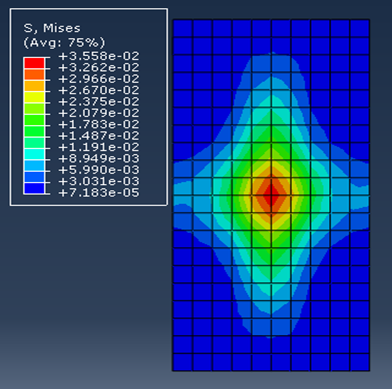
\includegraphics[width=0.7\linewidth,height=255pt]{Results/Point Loading/M6_VMS_L1_new.png} \\
  \end{tabular}
  \caption{Von Mises Stress (MPa) - Material 6, Load: 5N}
\end{figure}

\begin{figure}[H]
  \centering
  \begin{tabular}{@{}c@{}}
    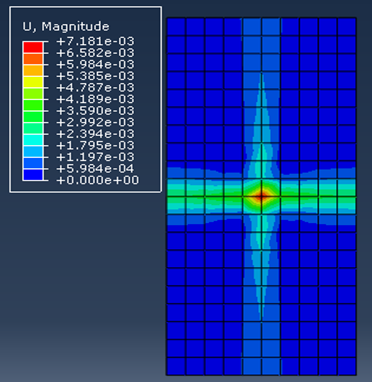
\includegraphics[width=0.7\linewidth,height=255pt]{Results/Point Loading/M6_DIS_L1_new.png} \\
  \end{tabular}
  \caption{Displacement (mm) - Material 6, Load: 5N}
\end{figure}

\begin{figure}[H]
  \centering
  \begin{tabular}{@{}c@{}}
    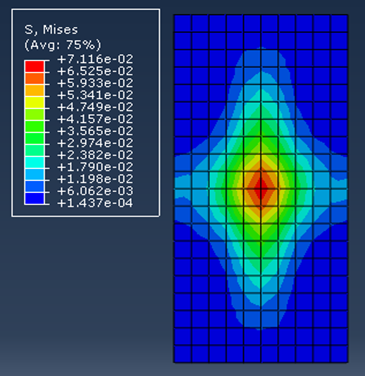
\includegraphics[width=0.7\linewidth,height=255pt]{Results/Point Loading/M6_VMS_L2_new.png} \\
  \end{tabular}
  \caption{Von Mises Stress (MPa) - Material 6, Load: 10N}
\end{figure}

\begin{figure}[H]
  \centering
  \begin{tabular}{@{}c@{}}
    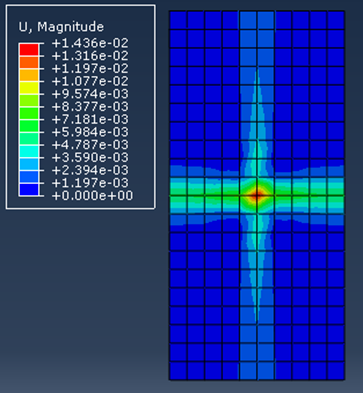
\includegraphics[width=0.7\linewidth,height=255pt]{Results/Point Loading/M6_DIS_L2_new.png} \\
  \end{tabular}
  \caption{Displacement (mm) - Material 6, Load: 10N}
\end{figure}

\begin{figure}[H]
  \centering
  \begin{tabular}{@{}c@{}}
    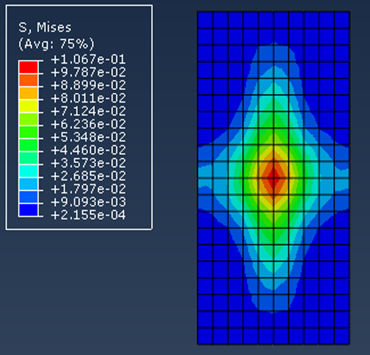
\includegraphics[width=0.7\linewidth,height=255pt]{Results/Point Loading/M6_VMS_L3_new.png} \\
  \end{tabular}
  \caption{Von Mises Stress (MPa) - Material 6, Load: 15N}
\end{figure}

\begin{figure}[H]
  \centering
  \begin{tabular}{@{}c@{}}
    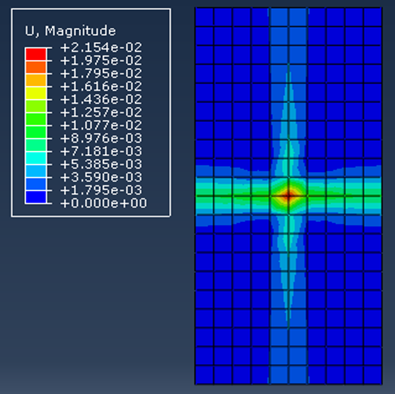
\includegraphics[width=0.7\linewidth,height=255pt]{Results/Point Loading/M6_DIS_L3_new.png} \\
  \end{tabular}
  \caption{Displacement (mm) - Material 6, Load: 15N}
\end{figure}

\begin{figure}[H]
  \centering
  \begin{tabular}{@{}c@{}}
    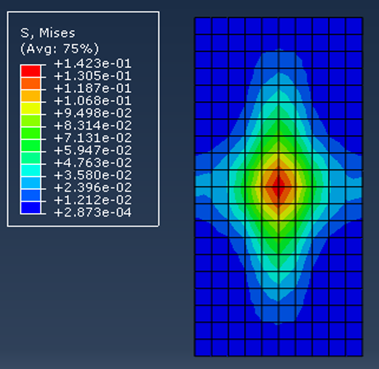
\includegraphics[width=0.7\linewidth,height=255pt]{Results/Point Loading/M6_VMS_L4_new.png} \\
  \end{tabular}
  \caption{Von Mises Stress (MPa) - Material 6, Load: 20N}
\end{figure}

\begin{figure}[H]
  \centering
  \begin{tabular}{@{}c@{}}
    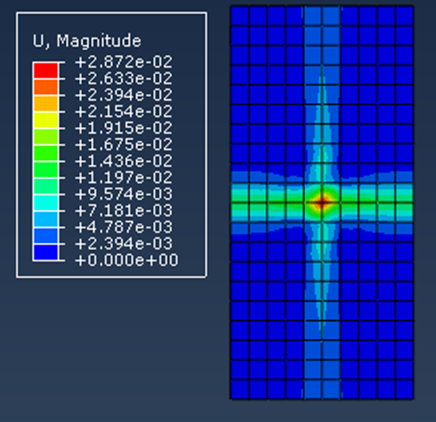
\includegraphics[width=0.7\linewidth,height=255pt]{Results/Point Loading/M6_DIS_L4_new.png} \\
  \end{tabular}
  \caption{Displacement (mm) - Material 6, Load: 20N}
\end{figure}

\begin{figure}[H]
  \centering
  \begin{tabular}{@{}c@{}}
    \includegraphics[width=0.7\linewidth,height=255pt]{Results/Point Loading/M6_VMS_L5_new.png} \\
  \end{tabular}
  \caption{Von Mises Stress (MPa) - Material 6, Load: 25N}
\end{figure}

\begin{figure}[H]
  \centering
  \begin{tabular}{@{}c@{}}
    \includegraphics[width=0.7\linewidth,height=255pt]{Results/Point Loading/M6_DIS_L5_new.png} \\
  \end{tabular}
  \caption{Displacement (mm) - Material 6, Load: 25N}
\end{figure}

%-------------------------------------------------------------------------------------------------------

\newpage
\noindent Material 6 - Bending Analysis 
\begin{figure}[H]
  \centering
  \begin{tabular}{@{}c@{}}
    \includegraphics[width=0.7\linewidth,height=255pt]{Results/Bending/M6_VMS_15_new.png} \\
  \end{tabular}
  \caption{Von Mises Stress (MPa) - Material 6,  Bending Angle: 15$^{\circ}$ }
\end{figure}

\begin{figure}[H]
  \centering
  \begin{tabular}{@{}c@{}}
    \includegraphics[width=0.7\linewidth,height=255pt]{Results/Bending/M6_DIS_15_new.png} \\
  \end{tabular}
  \caption{Displacement (mm) - Material 6, Bending Angle: 15$^{\circ}$ }
\end{figure}

\begin{figure}[H]
  \centering
  \begin{tabular}{@{}c@{}}
    \includegraphics[width=0.7\linewidth,height=255pt]{Results/Bending/M6_VMS_30_new.png} \\
  \end{tabular}
  \caption{Von Mises Stress (MPa) - Material 6,  Bending Angle: 30$^{\circ}$ }
\end{figure}

\begin{figure}[H]
  \centering
  \begin{tabular}{@{}c@{}}
    \includegraphics[width=0.7\linewidth,height=255pt]{Results/Bending/M6_DIS_30_new.png} \\
  \end{tabular}
  \caption{Displacement (mm) - Material 6, Bending Angle: 30$^{\circ}$ }
\end{figure}

\begin{figure}[H]
  \centering
  \begin{tabular}{@{}c@{}}
    \includegraphics[width=0.7\linewidth,height=255pt]{Results/Bending/M6_VMS_45_new.png} \\
  \end{tabular}
  \caption{Von Mises Stress (MPa) - Material 6,  Bending Angle: 45$^{\circ}$ }
\end{figure}

\begin{figure}[H]
  \centering
  \begin{tabular}{@{}c@{}}
    \includegraphics[width=0.7\linewidth,height=255pt]{Results/Bending/M6_DIS_45_new.png} \\
  \end{tabular}
  \caption{Displacement (mm) - Material 6, Bending Angle: 45$^{\circ}$ }
\end{figure}

\begin{figure}[H]
  \centering
  \begin{tabular}{@{}c@{}}
    \includegraphics[width=0.7\linewidth,height=255pt]{Results/Bending/M6_VMS_60_new.png} \\
  \end{tabular}
  \caption{Von Mises Stress (MPa) - Material 6,  Bending Angle: 60$^{\circ}$ }
\end{figure}

\begin{figure}[H]
  \centering
  \begin{tabular}{@{}c@{}}
    \includegraphics[width=0.7\linewidth,height=255pt]{Results/Bending/M6_DIS_60_new.png} \\
  \end{tabular}
  \caption{Displacement (mm) - Material 6, Bending Angle: 60$^{\circ}$ }
\end{figure}

\begin{figure}[H]
  \centering
  \begin{tabular}{@{}c@{}}
    \includegraphics[width=0.7\linewidth,height=255pt]{Results/Bending/M6_VMS_90_new.png} \\
  \end{tabular}
  \caption{Von Mises Stress (MPa) - Material 6,  Bending Angle: 90$^{\circ}$ }
\end{figure}

\begin{figure}[H]
  \centering
  \begin{tabular}{@{}c@{}}
    \includegraphics[width=0.7\linewidth,height=255pt]{Results/Bending/M6_DIS_90_new.png} \\
  \end{tabular}
  \caption{Displacement (mm) - Material 6, Bending Angle: 90$^{\circ}$ }
\end{figure}

\newpage
\subsection{Graphs}

\begin{figure}[H]
  \centering
  \begin{tabular}{@{}c@{}}
    \includegraphics[width=1\linewidth,height=250pt]{{Figures/Graph1.png}} \\
  \end{tabular}
  \caption{Graph of Maximum Stress at Various Loadings for All Materials}
\end{figure}

\begin{figure}[H]
  \centering
  \begin{tabular}{@{}c@{}}
    \includegraphics[width=1\linewidth,height=250pt]{{Figures/Graph2.png}} \\
  \end{tabular}
  \caption{Graph of Maximum Displacement at Various Loadings for All Materials}
\end{figure}

\begin{figure}[H]
  \centering
  \begin{tabular}{@{}c@{}}
    \includegraphics[width=1\linewidth,height=250pt]{{Figures/Graph3.png}} \\
  \end{tabular}
  \caption{Graph of Maximum Stress at Various Bending Angles for All Materials}
\end{figure}

\begin{figure}[H]
  \centering
  \begin{tabular}{@{}c@{}}
    \includegraphics[width=1\linewidth,height=250pt]{{Figures/Graph4.png}} \\
  \end{tabular}
  \caption{\centering Graph of Maximum Displacement at Various Bending Angles for All Materials}
\end{figure}

\newpage
\section{Discussions}

\subsection{Which Screen Performed the Best?}

\noindent Based on the graphs in Figures 4.41 to 4.44, all of the six materials have stresses within the elastic range, and none of them fail under given circumstances. This concludes that they are in a safer region. All materials 1-5 exhibit the highest values of maximum stress in the point loading case and lower maximum displacement values against increasing point load. Material 6 presents the highest value for maximum displacement, but slightly lower maximum stress values as load increases than other materials. This is because the Poisson’s ratio was the same in all graphene composite materials and different in material 6. Moreover, the graphs in Figures 4.43 and 4.44 illustrate how stress and displacement values increase along with bending angle in all materials, but material 6 has greater maximum stresses than graphene composite materials because it is much stronger and thus is more resistant to bending at required angles.

\subsection{Comparing Graphene Composite and Indium Tin Oxide}

\noindent Based on the observation from Figures 4.41 to 4.44, it can be concluded that ITO is a better material compared to graphene composite. Since both the point loading and the bending angle cases have yielded consistent results for the ITO, there has been no error and no unusual results. In contrast, graphene composite materials (1-5) are not very accurate as their results are entirely different; this is the main difference. The materials' production methods also impact this as different parameter values for each method provide very different effects on the results. Overall, ITO has shown that it is the best material choice for mobile screens, but with improved production techniques and more experiments, graphene composite will certainly alter this. It is important to conduct further testing and research to assess the detailed comparison between the two materials. Because graphene's screens are challenging to design and simulate, this is still not a viable commercial product. However, it may become one by finding ways to improve its qualities to replace ITO.

\subsection{How Accurate Is the Data Obtained for the Mobile Screens?}

\noindent The data gathered on mobile screens is somewhat accurate, but many anomalies and errors remain. The applied load on the screens, the induced stress, is only determined by the magnitude of the load and the resistance offered by the surface. Hence, the only difference will be in the deflection or deformation caused by the stronger material and the weaker material. As can be seen, the induced stresses for each material type against a specific load magnitude are the same for graphene composite materials, and the only difference is that we get less deformation and displacement in stronger materials and more deformation or displacement in weaker materials (which have a low young modulus).\vspace{\baselineskip}

\noindent Moreover, in bending, the induced stresses rise with increasing bending angle. However, the variation in stress for a particular angle cannot be seen since the cross-sectional area, the induced displacement, and all boundary conditions remain the same.\vspace{\baselineskip}

\noindent Furthermore, during the computational process, the screen height used is the diagonal height (165.1mm instead of 158.0mm), this does not affect the results, but it does not replicate the size of the screen to which reference was made.

\subsection{Do the Results Align With the Future Demand?}

\noindent It was found that the results of the analysis were generally in line with the future market. Still, only minimal data was analysed, and the computation procedure did not appear to be highly accurate overall. However, given graphene's impact on the industry for the past 20 years, it clearly aligns with future demand because the material data was acquired through ongoing scientific experiments that suggest scalable production of graphene composites.

\subsection{Limitations and Improvements}

\noindent Essentially, the screen was so simple it could have been achieved directly within Abaqus CAE without the need for extra software. For this reason, Abaqus CAE was used for modelling the screens instead of Autodesk Fusion 360.\vspace{\baselineskip}

Moreover, using independent instances was that they could take up too much memory, which meant that the software often crashed and caused errors. When Abaqus CAE references independent parts, it does not use the instantiation structure in the input file. Instead, it refers to a set of nodal coordinates and element connectivity.\vspace{\baselineskip}

\noindent In the FEM analysis, the point loading and bending angles should have been increased to understand better which of the screens had failed in the higher load and bending conditions. To see the full comprehensive analysis of the screens, the mesh type should have been changed for the modelling analysis. The element sizes would be varied through changes in the global seed density, changing element types from quadrilaterals to triangular and quadrilateral-dominated mesh elements, and finally changing the polynomial order from linear to quadratic.

\subsubsection{Issue Obtaining Properties Data}

\noindent GRANTA EduPack software and scientific journals were to be used to collect the properties data. However, during the research period, data on graphene composites and nanocomposite materials were not available on GRANTA EduPack. GRANT MI was the only commercialised software available to show the data, and it was not available to students, which delayed and brought errors to the computer simulation. Consequently, information was only available via scientific journals or review papers, which were mostly paid or offered limited access even with university credentials.\vspace{\baselineskip}

\noindent Graphene composites 1-5 are not even readily available on a large scale which means finding materials with the same production process was impossible. This meant that computational experiments relied on limited data available; thus, the computation experiment was not accurate, as there were no counterpart materials to compare. Further, this means that these screens will not behave in the same manner as the simulation model in a real-world scenario. This is because the simulation model represents the behaviour of the screens after conducting a theoretical analysis, and as such, the simulation might have errors, which reduces its accuracy.\vspace{\baselineskip}

\noindent An average value of Poisson’s ratio was used since the value for all the materials was unavailable. Since all graphene composite materials have the exact Poisson’s ratio, which is not the case in a real-life scenario, the results are not reliable, and further research is required.

\subsubsection{Problem Testing Conductivity and Transparency}

\noindent With Abaqus CAE’s limited capabilities, it was not possible to conduct the screens conductivity and transparency analysis; for this reason, a third software program was necessary to analyse the conductivity and transparency of a simulated screen. This information was left out of the report due to the time frame and the lack of understanding about potential software for these applications. Thus, if such tests were carried out, the results would have been more trustworthy and better compared with a typical mobile touchscreen. The result of this is that only half of the simulations were done, 120 instead of 240.

\subsubsection{Alternative Uses for Graphene Composites}

\noindent Based on the results obtained, graphene composites may be used as an alternative to other applications. There was no conductivity or transparency analysis performed; therefore, no determination can be made how the screens would behave if these analyses were done. Furthermore, graphene composites can potentially be used in applications such as the kindle, which is low-powered, portable, and easy to hold because of its small weight. Watches can also benefit from graphene properties. The casing for the watches can be made from graphene, making them robust yet lightweight. Since graphene is flexible, the straps of the watches could be made from graphene.\vspace{\baselineskip}

Finally, the modelling of flexible displays could be improved if a whole phone made of graphene were modelled. This would be a complete test for the mechanical component and would make the simulation data more reliable and accurate. Nevertheless, this would require plenty of data and information and substantial computational power to perform all the simulations.

\newpage
\section{Conclusions}

\noindent The overall objective of this report was to compare graphene composites and ITO screens by way of FEM simulation and discuss their production techniques. Based on this result, graphene composite screens may become an alternative to ITO as a transparent electrode in mobile screens that are used today. Even though the report follows the aims and objectives in line, integrating graphene composite into a mobile phone is not easy. There is a significant amount of science involved in creating an accurate, reliable, and working graphene composite mobile screen. The report discusses these composite materials' complicated and unique production processes using literature review and computational simulation. No data is available that repeats the experimental method on the chosen material, and no information is available regarding the quality of the graphene used. Therefore, to have graphene composites used in mobile phones or any alternative products, it is essential to conduct continuous research and experimentation with graphene composites and compare the behaviour of graphene composites with that of ITO. Graphene is undoubtedly a material that will enhance the ‘mobile phone’ to something extraordinary with its flexibility, strength, conductivity, and transparency properties.

%TC:ignore
\newpage
\section*{\centering Acknowledgements}
\phantomsection
\addcontentsline{toc}{section}{Acknowledgements}

\noindent All credit goes to Allah (SWT) and my family for making all of this possible and for giving me the knowledge and strength to handle both challenges and difficulties. Dr. Patrick Cullen provided support and guidance through our weekly meetings during the project. Throughout his meetings, I gained insight into many different aspects of writing and found appropriate ways to find sources and format them correctly. He has taken the time and put in the effort to inform other students and me how to write a good report for the final year, and I greatly appreciate all the knowledge I have gained from him.

\newpage
\section*{\centering Circumstances}
\phantomsection
\addcontentsline{toc}{section}{Circumstances}

\noindent At the same time I was researching this report, the ongoing COVID-19 pandemic made my working environment even more challenging. Living in an overcrowded and noisy household made it even harder to concentrate, especially since there was minimal quiet space at home. My family and I had also tested positive for COVID-19, which made it difficult for me to focus since I was more worried about my elderly parents, especially mum, whose health had progressively worsened at one time. Unfortunately, my dad had suffered from a heart attack, which meant I had to prioritise taking care of my siblings while my dad was in the hospital. I originally intended to collect experimental data at a lab, but it wasn't easy to conduct this project due to government guidelines and living far from the university.

\newpage
\section*{References}
\phantomsection
\addcontentsline{toc}{section}{References}

\noindent 360researchreports.com. (2020). Global Indium Tin Oxide Market – Industry Reports. [online] Available at: \url{https://www.360researchreports.com/global-indium-tin-oxide-market-15085363} [Accessed 28 Apr. 2021]\vspace{\baselineskip}

\noindent Acs.org. (2021). Are There Fundamental Limitations on the Sheet Resistance and Transmittance of Thin Graphene Films? [online] Available at: \url{https://pubs.acs.org/doi/10.1021/nn100343f} [Accessed 23 Apr. 2021]\vspace{\baselineskip}

\noindent Asif, K. (2020). GRAPHENE FROM GRAPHITE AND APPLICATION IN FLEXIBLE DISPLAYS. [online] QMPLUS: DEN318 - RAO: Queen Mary University of London. Available at: \url{https://qmplus.qmul.ac.uk/course/view.php?id=15298} [Accessed 10 Mar. 2021]\vspace{\baselineskip}

\noindent Avouris, P. and Dimitrakopoulos, C. (2012). Graphene: synthesis and applications. Materials Today, [online] 15(3), pp.86–97. Available at \url{https://www.sciencedirect.com/science/article/pii/S1369702112700445} [Accessed 21 Apr. 2021]\vspace{\baselineskip}

\noindent Bae, S., Kim, H., Lee, Y., Xu, X., Park, J.-S., Zheng, Y., Balakrishnan, J., Lei, T., Ri Kim, H., Song, Y.I., Kim, Y.-J., Kim, K.S., Özyilmaz, B., Ahn, J.-H., Hong, B.H. and Iijima, S. (2010). Roll-to-roll production of 30-inch graphene films for transparent electrodes. Nature Nanotechnology, [online] 5(8), pp.574–578. Available at: \url{https://www.nature.com/articles/nnano.2010.132#rightslink} [Accessed 24 Apr. 2021]\vspace{\baselineskip}

\noindent Bhuyan, Md.S.A., Uddin, Md.N., Islam, Md.M., Bipasha, F.A. and Hossain, S.S. (2016). Synthesis of graphene. International Nano Letters, [online] 6(2), pp.65–83. Available at: \url{https://link.springer.com/article/10.1007/s40089-015-0176-1/figures/2} [Accessed 21 Apr. 2021]\vspace{\baselineskip}

\noindent Bu.edu. (2021). Mechanics of Materials: Strain Mechanics of Slender Structures | Boston University. [online] Available at: \url{https://www.bu.edu/moss/mechanics-of-materials-strain/} [Accessed 26 Apr. 2021]\vspace{\baselineskip}

\noindent Bu.edu. (2021). Mechanics of Materials: Stress Mechanics of Slender Structures | Boston University. [online] Available at: \url{https://www.bu.edu/moss/mechanics-of-materials-stress/} [Accessed 26 Apr. 2021]\vspace{\baselineskip}

\noindent Businesswire.com. (2020). Global Touch Screen Displays Market 2020-2027 - Increasing Penetration of Mobile Devices Presents Enormous Growth Potential - ResearchAndMarkets.com. [online] Available at: \url{https://www.businesswire.com/news/home/20200708005693/en/Global-Touch-Screen-Displays-Market-2020-2027} [Accessed 8 Nov. 2020]\vspace{\baselineskip}

\noindent Cqmxi.com. (2019). Chongqing Graphene Technology. [online] Available at: \url{http://www.cqmxi.com/archives1201.html} [Accessed 23 Apr. 2021]\vspace{\baselineskip}

\noindent Device Specifications. (2012). Apple iPhone 11 Pro Max - Specifications. [online] Available at: \url{https://www.devicespecifications.com/en/model/47695219} [Accessed 20 Mar. 2021]\vspace{\baselineskip}

\noindent D’urso, L., Forte, G., Russo, P. and O. Puglisi (2011). Surface-enhanced Raman Scattering Study on 1D-2D Graphene-based Structures. [online] ResearchGate. Available at: \url{https://www.researchgate.net/publication/241088969_Surface-enhanced_Raman_Scattering_Study_on_1D-2D_Graphene-based_Structures} [Accessed 23 Apr. 2021]\vspace{\baselineskip}

\noindent Du, X., Skachko, I., Barker, A. and Andrei, E.Y. (2008). Approaching ballistic transport in suspended graphene. Nature Nanotechnology, [online] 3(8), pp.491–495. Available at: \url{https://www.nature.com/articles/nnano.2008.199} [Accessed 8 Nov. 2020]\vspace{\baselineskip} 

\noindent G Chiarotti and P Chiaradia (2018). Physics of Solid Surfaces Subvolume B. [online] Berlin, Heidelberg Springer Berlin Heidelberg. Available at: \url{https://materials.springer.com/bp/docs/978-3-662-53908-8} [Accessed 23 Apr. 2021]\vspace{\baselineskip}

\noindent Graphene: Composite Materials (2020). Composites and coatings - Graphene - The University of Manchester. [online] Manchester.ac.uk. Available at: \url{https://www.graphene.manchester.ac.uk/learn/applications/composites-and-coatings/} [Accessed 4 Nov. 2020]\vspace{\baselineskip}

\noindent Graphene-info.com. (2017). Graphene-Info. [online] Available at: \url{https://www.graphene-info.com/graphene-mobile-industry} [Accessed 10 Apr. 2021]\vspace{\baselineskip}

\noindent Graphenesq.com. (2014). GRAPHENE SQUARE. [online] Available at: \url{http://www.graphenesq.com/whatis/graphene.asp} [Accessed 30 Oct. 2020].\vspace{\baselineskip}

\noindent Hameed, N., Dumée, L.F., Allioux, F.-M., Reghat, M., Church, J.S., Naebe, M., Magniez, K., Parameswaranpillai, J. and Fox, B.L. (2018). Graphene based room temperature flexible nanocomposites from permanently cross-linked networks. Scientific Reports, [online] 8(1). Available at: \url{https://www.nature.com/articles/s41598-018-21114-5} [Accessed 14 Mar. 2021]\vspace{\baselineskip}

\noindent Intertek.com. (2011). Graphene Analysis and Quality Assurance. [online] Available at: \url{https://www.intertek.com/chemicals/graphene-analysis/} [Accessed 8 Nov. 2020]\vspace{\baselineskip}

\noindent Jesus (2020). Properties of Graphene. [online] Graphenea. Available at: \url{ https://www.graphenea.com/pages/graphene-properties\#.X6Rpboj7RhE} [Accessed 1 Nov. 2020]\vspace{\baselineskip}

\noindent Kauling, A.P., Seefeldt, A.T., Pisoni, D.P., Pradeep, R.C., Bentini, R., Oliveira, R.V.B., Novoselov, K.S. and Castro Neto, A.H. (2018). The Worldwide Graphene Flake Production. Advanced Materials, [online] 30(44), p.1803784. Available at: \url{https://onlinelibrary.wiley.com/doi/abs/10.1002/adma.201803784} [Accessed 24 Apr. 2021]\vspace{\baselineskip}

\noindent Kim, K.S., Zhao, Y., Jang, H., Lee, S.Y., Kim, J.M., Kim, K.S., Ahn, J.-H., Kim, P., Choi, J.-Y. and Hong, B.H. (2009). Large-scale pattern growth of graphene films for stretchable transparent electrodes. Nature, [online] 457(7230), pp.706–710. Available at: \url{https://pubmed.ncbi.nlm.nih.gov/19145232/} [Accessed 23 Apr. 2021]\vspace{\baselineskip}

\noindent Kim, Y., Lee, J., Yeom, M.S., Shin, J.W., Kim, H., Cui, Y., Kysar, J.W., Hone, J., Jung, Y., Jeon, S. and Han, S.M. (2013). Strengthening effect of single-atomic-layer graphene in metal–graphene nanolayered composites. Nature Communications, [online] 4(1). Available at: \url{https://www.nature.com/articles/ncomms3114} [Accessed 25 Mar. 2021]\vspace{\baselineskip}

\noindent King, H.M. (2012). Graphite: A mineral with extreme properties and many uses. [online] Geology.com. Available at: \url{https://geology.com/minerals/graphite.shtml} [Accessed 1 Nov. 2020]\vspace{\baselineskip}

\noindent Kong, W., Kum, H., Bae, S.-H., Shim, J., Kim, H., Kong, L., Meng, Y., Wang, K., Kim, C. and Kim, J. (2019). Path towards graphene commercialization from lab to market. Nature Nanotechnology, [online] 14(10), pp.927–938. Available at: https://www.nature.com/articles/s41565-019-0555-2 [Accessed 21 Apr. 2021] \vspace{\baselineskip}

\noindent Lee, C., Wei, X., Kysar, J.W. and Hone, J. (2008). Measurement of the Elastic Properties and Intrinsic Strength of Monolayer Graphene. Science, [online] 321(5887), pp.385–388. Available at: \url{https://pubmed.ncbi.nlm.nih.gov/18635798/} [Accessed 23 Apr. 2021]\vspace{\baselineskip}

\noindent Lee, H.-S., Bang, J.-O., Lee, H.-J., Lee, G.-J., Chai, K.-H. and Jung, S.-B. (2011). Analysis of thermo-mechanical behavior of ITO layer on PET substrate. 2011 IEEE 61st Electronic Components and Technology Conference (ECTC). [online] Available at: \url{https://ieeexplore.ieee.org/document/5898757} [Accessed 14 Mar. 2021]\vspace{\baselineskip}

\noindent Lee, T.-W. (2020). Graphene for flexible lighting and displays. Duxford, United Kingdom Woodhead Publishing, p.14.\vspace{\baselineskip}

\noindent Lee, T.-W. (2020). Graphene for flexible lighting and displays. Duxford, United Kingdom Woodhead Publishing, p.8.\vspace{\baselineskip}

\noindent Lee, T.-W. (2020). Graphene for flexible lighting and displays. Duxford, United Kingdom Woodhead Publishing, p.175. - p.176.\vspace{\baselineskip}

\noindent Liang, K., Spiesz, E.M., Schmieden, D.T., Xu, A.-W., Meyer, A.S. and Aubin-Tam, M.-E. (2020). Bioproduced Polymers Self-Assemble with Graphene Oxide into Nanocomposite Films with Enhanced Mechanical Performance. ACS Nano, 14(11), pp.14731–14739 [online] Available at: \url{https://pubs.acs.org/doi/10.1021/acsnano.0c00913} [Accessed 14 Mar. 2021]\vspace{\baselineskip}

\noindent Liu, N., Chortos, A., Lei, T., Jin, L., Kim, T.R., Bae, W.-G., Zhu, C., Wang, S., Pfattner, R., Chen, X., Sinclair, R. and Bao, Z. (2017). Ultratransparent and stretchable graphene electrodes. Science Advances, [online] 3(9), p.e1700159. Available at: \url{https://pubmed.ncbi.nlm.nih.gov/28913422/} [Accessed 23 Apr. 2021]\vspace{\baselineskip}

\noindent Ma, Y.Z., Sobernheim, D. and Garzon, J.R. (2016). Glossary for Unconventional Oil and Gas Resource Evaluation and Development. Unconventional Oil and Gas Resources Handbook, [online] pp.513–526. Available at: \url{https://www.sciencedirect.com/science/article/pii/B9780128022382000195} [Accessed 26 Apr. 2021]\vspace{\baselineskip}

\noindent Michael Berger (2015). What is Graphene? Graphene properties and applications. [online] Nanowerk. Available at: \url{https://www.nanowerk.com/what\_is\_graphene.php} [Accessed 30 Oct. 2020].\vspace{\baselineskip}

\noindent Muñoz, R. and Gómez-Aleixandre, C. (2013). Review of CVD Synthesis of Graphene. Chemical Vapor Deposition, [online] 19(10-11-12), pp.297–322. Available at: \url{https://onlinelibrary.wiley.com/doi/abs/10.1002/cvde.201300051} [Accessed 23 Apr. 2021]\vspace{\baselineskip}

\noindent Nair, R.R., Blake, P., Grigorenko, A.N., Novoselov, K.S., Booth, T.J., Stauber, T., Peres, N.M.R. and Geim, A.K. (2008). Fine Structure Constant Defines Visual Transparency of Graphene. Science, [online] 320(5881), pp.1308–1308. Available at: \url{https://science.sciencemag.org/content/320/5881/1308} [Accessed 23 Apr. 2021]\vspace{\baselineskip}

\noindent Novoselov, K.S. (2004). Electric Field Effect in Atomically Thin Carbon Films. Science, [online] 306(5696), pp.666–669. Available at: \url{https://pubmed.ncbi.nlm.nih.gov/15499015/} [Accessed 21 Apr. 2021]\vspace{\baselineskip}

\noindent Rafiee, M.A., Rafiee, J., Wang, Z., Song, H., Yu, Z.-Z. and Koratkar, N. (2009). Enhanced Mechanical Properties of Nanocomposites at Low Graphene Content. ACS Nano, 3(12), pp.3884–3890. Available at: \url{https://pubs.acs.org/doi/pdf/10.1021/nn9010472} [Accessed 14 Mar. 2020].\vspace{\baselineskip}

\noindent Ryu, J., Kim, Y., Won, D., Kim, N., Park, J.S., Lee, E.-K., Cho, D., Cho, S.-P., Kim, S.J., Ryu, G.H., Shin, H.-A.-S., Lee, Z., Hong, B.H. and Cho, S. (2014). Fast Synthesis of High-Performance Graphene Films by Hydrogen-Free Rapid Thermal Chemical Vapor Deposition. ACS Nano, [online] 8(1), pp.950–956. Available at: \url{https://pubmed.ncbi.nlm.nih.gov/24358985/} [Accessed 23 Apr. 2021]\vspace{\baselineskip}

\noindent Sang, M., Shin, J., Kim, K. and Yu, K. (2019). Electronic and Thermal Properties of Graphene and Recent Advances in Graphene Based Electronics Applications. Nanomaterials, [online] 9(3), p.374. Available at: \url{https://www.ncbi.nlm.nih.gov/pmc/articles/PMC6474003/} [Accessed 1 Nov. 2020].\vspace{\baselineskip}

\noindent Sheehy, D.E. and Schmalian, J. (2009). Optical transparency of graphene as determined by the fine-structure constant. Physical Review B, [online] 80(19). Available at: \url{https://journals.aps.org/prb/abstract/10.1103/PhysRevB.80.193411} [Accessed 31 Oct. 2020].\vspace{\baselineskip}

\noindent Sigma-Aldrich, 752657 (2017). Indium tin oxide 752657. [online] Available at: \url{https://www.sigmaaldrich.com/catalog/product/aldrich/752657} [Accessed 26 Apr. 2021]\vspace{\baselineskip}

\noindent SimScale. (2021). What is Von Mises Stress? | SimScale Finite Element Analysis. [online] Available at: \url{https://www.simscale.com/docs/simwiki/fea-finite-element-analysis/what-is-von-mises-stress/} [Accessed 26 Apr. 2021]\vspace{\baselineskip}

\noindent Sirois, S. (2018). How Do Touch Screens Work on Laptops and Tablets? [online] Hp.com. Available at: \url{https://store.hp.com/us/en/tech-takes/how-do-touch-screens-work} [Accessed 8 Nov. 2020]\vspace{\baselineskip}

\noindent Stankovich, S., Dikin, D.A., Dommett, G.H.B., Kohlhaas, K.M., Zimney, E.J., Stach, E.A., Piner, R.D., Nguyen, S.T. and Ruoff, R.S. (2006). Graphene-based composite materials. Nature, [online] 442(7100), pp.282–286. Available at: \url{https://www.nature.com/articles/nature04969} [Accessed 5 Apr. 2021]\vspace{\baselineskip}

\noindent Statista. (2020). Number of mobile devices worldwide 2020-2024 | Statista. [online] Available at: \url{https://www.statista.com/statistics/245501/multiple-mobile-device-ownership-worldwide/} [Accessed 12 Nov. 2020].\vspace{\baselineskip}

\noindent The American Ceramic Society (2018). Poor quality (or fake) graphene could be hindering your research | The American Ceramic Society. [online] The American Ceramic Society. Available at: \url{https://ceramics.org/ceramic-tech-today/raw-materials-supply/poor-quality-or-fake-graphene-could-be-hindering-your-research} [Accessed 8 Nov. 2020]\vspace{\baselineskip}

\noindent Tirupatigraphite.com. (2017). Flake Graphite Experts From India. [online] Available at: \url{http://tirupatigraphite.com/about\_flake\_graphite.html\#} [Accessed 7 Nov. 2020]\vspace{\baselineskip}

\noindent Universe-review.ca. (2018). Graphene. [online] Available at: \url{https://universe-review.ca/R13-16-graphene.htm} [Accessed 6 Nov. 2020]\vspace{\baselineskip}

\noindent Usgs.gov. (2021). Indium Statistics and Information. [online] Available at: \url{https://www.usgs.gov/centers/nmic/indium-statistics-and-information} [Accessed 22 Mar. 2021]\vspace{\baselineskip}

\noindent Won, S., Hwangbo, Y., Lee, S.-K., Kim, K.-S., Kim, K.-S., Lee, S.-M., Lee, H.-J., Ahn, J.-H., Kim, J.-H. and Lee, S.-B. (2014). Double-layer CVD graphene as stretchable transparent electrodes. Nanoscale, [online] 6(11), pp.6057–6064. Available at: \url{https://pubs.rsc.org/az/content/articlelanding/2014/nr/c4nr00265b#!divAbstract} [Accessed 23 Apr. 2021]\vspace{\baselineskip}

\noindent Xin Zhao (2017) - Mechanical Properties of Graphene and Graphene-based Nanocomposites. (n.d.). [online] . Available at: \url{https://www.research.manchester.ac.uk/portal/files/86864125/FULL_TEXT.PDF} [Accessed 14 Mar. 2021]\vspace{\baselineskip}

\noindent Zhan, Y., Xiong, C., Yang, J., Shi, Z. and Yang, Q. (2019). Flexible cellulose nanofibril/pristine graphene nanocomposite films with high electrical conductivity. Composites Part A: Applied Science and Manufacturing, [online] 119, pp.119–126. Available at: \url{https://www.sciencedirect.com/science/article/abs/pii/S1359835X19300351} [Accessed 14 Mar. 2021]\vspace{\baselineskip}

\noindent Zhang, J.J. (2019). Rock physical and mechanical properties. Applied Petroleum Geomechanics, [online] pp.29–83. Available at: \url{https://www.sciencedirect.com/science/article/pii/B9780128148143000022} [Accessed 26 Apr. 2021]\vspace{\baselineskip}

\noindent Zhu, Y., Ji, H., Cheng, H.-M. and Ruoff, R.S. (2017). Mass production and industrial applications of graphene materials. National Science Review, [online] 5(1), pp.90–101. Available at: \url{https://academic.oup.com/nsr/article/5/1/90/3861355} [Accessed 23 Apr. 2021]\vspace{\baselineskip}


\newpage
\section*{Appendix}
\phantomsection
\addcontentsline{toc}{section}{Appendix}

\noindent The raw material properties data used in the simulation analysis are presented below.

\begin{table}[hbt!]
\centering
\caption{Raw Properties of Material 1}
\begin{tabular}{|l|c|}
\hline
\multicolumn{2}{|c|}{\textbf{Material 1: Graphene Loading wt\% 0.6}} \\ \hline
Young's Modulus                   & 650 MPa                          \\ \hline
Tensile Strength                  & 35 MPa                           \\ \hline
Electrical Resistivity            & 35 k$\Omega$m                    \\ \hline
Reference                         & (Hameed et al., 2018)            \\ \hline
\end{tabular}
\end{table}

\begin{table}[hbt!]
\centering
\caption{Raw Properties of Material 2}
\begin{tabular}{|l|c|}
\hline
\multicolumn{2}{|c|}{\textbf{Material 2: Graphene content 10 - TOCN-RGO}} \\ \hline
Young's Modulus                       & 8.4 GPa                           \\ \hline
Tensile Strength                      & 425 MPa                           \\ \hline
Elongation at Break                   & 20\%                              \\ \hline
Electrical Conductivity               & 0.75 Scm$^-1$                     \\ \hline
Reference                             & (Zhan et al., 2019)               \\ \hline
\end{tabular}
\end{table}

\begin{table}[hbt!]
\centering
\caption{Raw Properties of Material 3}
\begin{tabular}{|l|c|}
\hline
\multicolumn{2}{|c|}{\textbf{Material 3: Bioinspired films PGA/GO/Ca$^{2+}$}} \\ \hline
Young's Modulus  & $21.4\pm{8.7}$ GPa \\ \hline
Tensile Strength & $150\pm51.9$ MPa   \\ \hline
Reference        & (Liang et al., 2020)   \\ \hline
\end{tabular}
\end{table}

\FloatBarrier
\begin{table}[hbt!]
\centering
\caption{Raw Properties of Material 4}
\begin{tabular}{|l|c|}
\hline
\multicolumn{2}{|c|}{\textbf{Material 4: Graphene Reinforced Epoxy Nanocomposites EEG 0.05vol.\%}} \\ \hline
Young's Modulus     & 2.52 GPa         \\ \hline
Tensile Strength    & 42.5 MPa         \\ \hline
Elongation at Break & 2.2\%            \\ \hline
Reference           & (Xin Zhao, 2017) \\ \hline
\end{tabular}
\end{table}
\FloatBarrier

\begin{table}[hbt!]
\centering
\caption{Raw Properties of Material 5}
\label{tab:my-table}
\begin{tabular}{|l|c|}
\hline
\multicolumn{2}{|c|}{\textbf{\begin{tabular}[c]{@{}c@{}}Material 5: Graphene Nanocomposites (0.1\% wt GPL)\end{tabular}}} \\ \hline
Young's Modulus  & 3.75 GPa              \\ \hline
Tensile Strength & 77 MPa                \\ \hline
Reference        & (Rafiee et al., 2009) \\ \hline
\end{tabular}
\end{table}

\begin{table}[hbt!]
\centering
\caption{Raw Properties of Material 6}
\begin{tabular}{|l|c|}
\hline
\multicolumn{2}{|c|}{\textbf{Material 6: Indium Tin Oxide}} \\ \hline
Young's Modulus & $119\pm5$ GPa                  \\ \hline
Density         & 14 gcm$^{-3}$ \\ \hline
Coefficient of Thermal Expansion (CTE) & {7.6 x 10$^{-6}$}     \\ \hline
Poisson's Ratio & 0.35                       \\ \hline
Reference       & (Lee et al., 2011)           \\ \hline
\end{tabular}
\end{table}

\newpage
\noindent Below are the results of a point loading and bending analysis on four screens, using four different material properties.\vspace{\baselineskip}

%-------------------------------------------------------------------------------------------------------

\noindent Material 2 - Point Loading 
\begin{figure}[H]
  \centering
  \begin{tabular}{@{}c@{}}
    \includegraphics[width=0.7\linewidth,height=255pt]{Results/Point Loading/M2_VMS_L1.png} \\
  \end{tabular}
  \caption{Von Mises Stress (MPa) - Material 2, Load: 5N}
\end{figure}

\begin{figure}[H]
  \centering
  \begin{tabular}{@{}c@{}}
    \includegraphics[width=0.7\linewidth,height=255pt]{Results/Point Loading/M2_DIS_L1.png} \\
  \end{tabular}
  \caption{Displacement (mm) - Material 2, Load: 5N}
\end{figure}

\begin{figure}[H]
  \centering
  \begin{tabular}{@{}c@{}}
    \includegraphics[width=0.7\linewidth,height=255pt]{Results/Point Loading/M2_VMS_L2.png} \\
  \end{tabular}
  \caption{Von Mises Stress (MPa) - Material 2, Load: 10N}
\end{figure}

\begin{figure}[H]
  \centering
  \begin{tabular}{@{}c@{}}
    \includegraphics[width=0.7\linewidth,height=255pt]{Results/Point Loading/M2_DIS_L2.png} \\
  \end{tabular}
  \caption{Displacement (mm) - Material 2, Load: 10N}
\end{figure}

\begin{figure}[H]
  \centering
  \begin{tabular}{@{}c@{}}
    \includegraphics[width=0.7\linewidth,height=255pt]{Results/Point Loading/M2_VMS_L3.png} \\
  \end{tabular}
  \caption{Von Mises Stress (MPa) - Material 2, Load: 15N}
\end{figure}

\begin{figure}[H]
  \centering
  \begin{tabular}{@{}c@{}}
    \includegraphics[width=0.7\linewidth,height=255pt]{Results/Point Loading/M2_DIS_L3.png} \\
  \end{tabular}
  \caption{Displacement (mm) - Material 2, Load: 15N}
\end{figure}

\begin{figure}[H]
  \centering
  \begin{tabular}{@{}c@{}}
    \includegraphics[width=0.7\linewidth,height=255pt]{Results/Point Loading/M2_VMS_L4.png} \\
  \end{tabular}
  \caption{Von Mises Stress (MPa) - Material 2, Load: 20N}
\end{figure}

\begin{figure}[H]
  \centering
  \begin{tabular}{@{}c@{}}
    \includegraphics[width=0.7\linewidth,height=255pt]{Results/Point Loading/M2_DIS_L4.png} \\
  \end{tabular}
  \caption{Displacement (mm) - Material 2, Load: 20N}
\end{figure}

\begin{figure}[H]
  \centering
  \begin{tabular}{@{}c@{}}
    \includegraphics[width=0.7\linewidth,height=255pt]{Results/Point Loading/M2_VMS_L5.png} \\
  \end{tabular}
  \caption{Von Mises Stress (MPa) - Material 2, Load: 25N}
\end{figure}

\begin{figure}[H]
  \centering
  \begin{tabular}{@{}c@{}}
    \includegraphics[width=0.7\linewidth,height=255pt]{Results/Point Loading/M2_DIS_L5.png} \\
  \end{tabular}
  \caption{Displacement (mm) - Material 2, Load: 25N}
\end{figure}

%------------------------------------------------------------------------------------------------------

\newpage
\noindent Material 3 - Point Loading 
\begin{figure}[H]
  \centering
  \begin{tabular}{@{}c@{}}
    \includegraphics[width=0.7\linewidth,height=255pt]{Results/Point Loading/M3_VMS_L1.png} \\
  \end{tabular}
  \caption{Von Mises Stress (MPa) - Material 3, Load: 5N}
\end{figure}

\begin{figure}[H]
  \centering
  \begin{tabular}{@{}c@{}}
    \includegraphics[width=0.7\linewidth,height=255pt]{Results/Point Loading/M3_DIS_L1.png} \\
  \end{tabular}
  \caption{Displacement (mm) - Material 3, Load: 5N}
\end{figure}

\begin{figure}[H]
  \centering
  \begin{tabular}{@{}c@{}}
    \includegraphics[width=0.7\linewidth,height=255pt]{Results/Point Loading/M3_VMS_L2.png} \\
  \end{tabular}
  \caption{Von Mises Stress (MPa) - Material 3, Load: 10N}
\end{figure}

\begin{figure}[H]
  \centering
  \begin{tabular}{@{}c@{}}
    \includegraphics[width=0.7\linewidth,height=255pt]{Results/Point Loading/M3_DIS_L2.png} \\
  \end{tabular}
  \caption{Displacement (mm) - Material 3, Load: 10N}
\end{figure}

\begin{figure}[H]
  \centering
  \begin{tabular}{@{}c@{}}
    \includegraphics[width=0.7\linewidth,height=255pt]{Results/Point Loading/M3_VMS_L3.png} \\
  \end{tabular}
  \caption{Von Mises Stress (MPa) - Material 3, Load: 15N}
\end{figure}

\begin{figure}[H]
  \centering
  \begin{tabular}{@{}c@{}}
    \includegraphics[width=0.7\linewidth,height=255pt]{Results/Point Loading/M3_DIS_L3.png} \\
  \end{tabular}
  \caption{Displacement (mm) - Material 3, Load: 15N}
\end{figure}

\begin{figure}[H]
  \centering
  \begin{tabular}{@{}c@{}}
    \includegraphics[width=0.7\linewidth,height=255pt]{Results/Point Loading/M3_VMS_L4.png} \\
  \end{tabular}
  \caption{Von Mises Stress (MPa) - Material 3, Load: 20N}
\end{figure}

\begin{figure}[H]
  \centering
  \begin{tabular}{@{}c@{}}
    \includegraphics[width=0.7\linewidth,height=255pt]{Results/Point Loading/M3_DIS_L4.png} \\
  \end{tabular}
  \caption{Displacement (mm) - Material 3, Load: 20N}
\end{figure}

\begin{figure}[H]
  \centering
  \begin{tabular}{@{}c@{}}
    \includegraphics[width=0.7\linewidth,height=255pt]{Results/Point Loading/M3_VMS_L5.png} \\
  \end{tabular}
  \caption{Von Mises Stress (MPa) - Material 3, Load: 25N}
\end{figure}

\begin{figure}[H]
  \centering
  \begin{tabular}{@{}c@{}}
    \includegraphics[width=0.7\linewidth,height=255pt]{Results/Point Loading/M3_DIS_L5.png} \\
  \end{tabular}
  \caption{Displacement (mm) - Material 3, Load: 25N}
\end{figure}

%-------------------------------------------------------------------------------------------

\newpage
\noindent Material 4 - Point Loading 
\begin{figure}[H]
  \centering
  \begin{tabular}{@{}c@{}}
    \includegraphics[width=0.7\linewidth,height=255pt]{Results/Point Loading/M4_VMS_L1.png} \\
  \end{tabular}
  \caption{Von Mises Stress (MPa) - Material 4, Load: 5N}
\end{figure}

\begin{figure}[H]
  \centering
  \begin{tabular}{@{}c@{}}
    \includegraphics[width=0.7\linewidth,height=255pt]{Results/Point Loading/M4_DIS_L1.png} \\
  \end{tabular}
  \caption{Displacement (mm) - Material 4, Load: 5N}
\end{figure}

\begin{figure}[H]
  \centering
  \begin{tabular}{@{}c@{}}
    \includegraphics[width=0.7\linewidth,height=255pt]{Results/Point Loading/M4_VMS_L2.png} \\
  \end{tabular}
  \caption{Von Mises Stress (MPa) - Material 4, Load: 10N}
\end{figure}

\begin{figure}[H]
  \centering
  \begin{tabular}{@{}c@{}}
    \includegraphics[width=0.7\linewidth,height=255pt]{Results/Point Loading/M4_DIS_L2.png} \\
  \end{tabular}
  \caption{Displacement (mm) - Material 4, Load: 10N}
\end{figure}

\begin{figure}[H]
  \centering
  \begin{tabular}{@{}c@{}}
    \includegraphics[width=0.7\linewidth,height=255pt]{Results/Point Loading/M4_VMS_L3.png} \\
  \end{tabular}
  \caption{Von Mises Stress (MPa) - Material 4, Load: 15N}
\end{figure}

\begin{figure}[H]
  \centering
  \begin{tabular}{@{}c@{}}
    \includegraphics[width=0.7\linewidth,height=255pt]{Results/Point Loading/M4_DIS_L3.png} \\
  \end{tabular}
  \caption{Displacement (mm) - Material 4, Load: 15N}
\end{figure}

\begin{figure}[H]
  \centering
  \begin{tabular}{@{}c@{}}
    \includegraphics[width=0.7\linewidth,height=255pt]{Results/Point Loading/M4_VMS_L4.png} \\
  \end{tabular}
  \caption{Von Mises Stress (MPa) - Material 4, Load: 20N}
\end{figure}

\begin{figure}[H]
  \centering
  \begin{tabular}{@{}c@{}}
    \includegraphics[width=0.7\linewidth,height=255pt]{Results/Point Loading/M4_DIS_L4.png} \\
  \end{tabular}
  \caption{Displacement (mm) - Material 4, Load: 20N}
\end{figure}

\begin{figure}[H]
  \centering
  \begin{tabular}{@{}c@{}}
    \includegraphics[width=0.7\linewidth,height=255pt]{Results/Point Loading/M4_VMS_L5.png} \\
  \end{tabular}
  \caption{Von Mises Stress (MPa) - Material 4, Load: 25N}
\end{figure}

\begin{figure}[H]
  \centering
  \begin{tabular}{@{}c@{}}
    \includegraphics[width=0.7\linewidth,height=255pt]{Results/Point Loading/M4_DIS_L5.png} \\
  \end{tabular}
  \caption{Displacement (mm) - Material 4, Load: 25N}
\end{figure}

%-------------------------------------------------------------------------------------------

\newpage
\noindent Material 5 - Point Loading 
\begin{figure}[H]
  \centering
  \begin{tabular}{@{}c@{}}
    \includegraphics[width=0.7\linewidth,height=255pt]{Results/Point Loading/M5_VMS_L1.png} \\
  \end{tabular}
  \caption{Von Mises Stress (MPa) - Material 5, Load: 5N}
\end{figure}

\begin{figure}[H]
  \centering
  \begin{tabular}{@{}c@{}}
    \includegraphics[width=0.7\linewidth,height=255pt]{Results/Point Loading/M5_DIS_L1.png} \\
  \end{tabular}
  \caption{Displacement (mm) - Material 5, Load: 5N}
\end{figure}

\begin{figure}[H]
  \centering
  \begin{tabular}{@{}c@{}}
    \includegraphics[width=0.7\linewidth,height=255pt]{Results/Point Loading/M5_VMS_L2.png} \\
  \end{tabular}
  \caption{Von Mises Stress (MPa) - Material 5, Load: 10N}
\end{figure}

\begin{figure}[H]
  \centering
  \begin{tabular}{@{}c@{}}
    \includegraphics[width=0.7\linewidth,height=255pt]{Results/Point Loading/M5_DIS_L2.png} \\
  \end{tabular}
  \caption{Displacement (mm) - Material 5, Load: 10N}
\end{figure}

\begin{figure}[H]
  \centering
  \begin{tabular}{@{}c@{}}
    \includegraphics[width=0.7\linewidth,height=255pt]{Results/Point Loading/M5_VMS_L3.png} \\
  \end{tabular}
  \caption{Von Mises Stress (MPa) - Material 5, Load: 15N}
\end{figure}

\begin{figure}[H]
  \centering
  \begin{tabular}{@{}c@{}}
    \includegraphics[width=0.7\linewidth,height=255pt]{Results/Point Loading/M5_DIS_L3.png} \\
  \end{tabular}
  \caption{Displacement (mm) - Material 5, Load: 15N}
\end{figure}

\begin{figure}[H]
  \centering
  \begin{tabular}{@{}c@{}}
    \includegraphics[width=0.7\linewidth,height=255pt]{Results/Point Loading/M5_VMS_L4.png} \\
  \end{tabular}
  \caption{Von Mises Stress (MPa) - Material 5, Load: 20N}
\end{figure}

\begin{figure}[H]
  \centering
  \begin{tabular}{@{}c@{}}
    \includegraphics[width=0.7\linewidth,height=255pt]{Results/Point Loading/M5_DIS_L4.png} \\
  \end{tabular}
  \caption{Displacement (mm) - Material 5, Load: 20N}
\end{figure}

\begin{figure}[H]
  \centering
  \begin{tabular}{@{}c@{}}
    \includegraphics[width=0.7\linewidth,height=255pt]{Results/Point Loading/M5_VMS_L5.png} \\
  \end{tabular}
  \caption{Von Mises Stress (MPa) - Material 5, Load: 25N}
\end{figure}

\begin{figure}[H]
  \centering
  \begin{tabular}{@{}c@{}}
    \includegraphics[width=0.7\linewidth,height=255pt]{Results/Point Loading/M5_DIS_L5.png} \\
  \end{tabular}
  \caption{Displacement (mm) - Material 5, Load: 25N}
\end{figure}

\newpage 
\noindent Below shows the simulation of screens undergoing bending analysis using different material properties of graphene.\vspace{\baselineskip}

%-------------------------------------------------------------------------------------------------------

\noindent Material 2 - Bending Analysis 
\begin{figure}[H]
  \centering
  \begin{tabular}{@{}c@{}}
    \includegraphics[width=0.7\linewidth,height=255pt]{Results/Bending/M2_VMS_15.png} \\
  \end{tabular}
  \caption{Von Mises Stress (MPa) - Material 2,  Bending Angle: 15$^{\circ}$ }
\end{figure}

\begin{figure}[H]
  \centering
  \begin{tabular}{@{}c@{}}
    \includegraphics[width=0.7\linewidth,height=255pt]{Results/Bending/M2_DIS_15.png} \\
  \end{tabular}
  \caption{Displacement (mm) - Material 2, Bending Angle: 15$^{\circ}$ }
\end{figure}

\begin{figure}[H]
  \centering
  \begin{tabular}{@{}c@{}}
    \includegraphics[width=0.7\linewidth,height=255pt]{Results/Bending/M2_VMS_30.png} \\
  \end{tabular}
  \caption{Von Mises Stress (MPa) - Material 2,  Bending Angle: 30$^{\circ}$ }
\end{figure}

\begin{figure}[H]
  \centering
  \begin{tabular}{@{}c@{}}
    \includegraphics[width=0.7\linewidth,height=255pt]{Results/Bending/M2_DIS_30.png} \\
  \end{tabular}
  \caption{Displacement (mm) - Material 2, Bending Angle: 30$^{\circ}$ }
\end{figure}

\begin{figure}[H]
  \centering
  \begin{tabular}{@{}c@{}}
    \includegraphics[width=0.7\linewidth,height=255pt]{Results/Bending/M2_VMS_45.png} \\
  \end{tabular}
  \caption{Von Mises Stress (MPa) - Material 2,  Bending Angle: 45$^{\circ}$ }
\end{figure}

\begin{figure}[H]
  \centering
  \begin{tabular}{@{}c@{}}
    \includegraphics[width=0.7\linewidth,height=255pt]{Results/Bending/M2_DIS_45.png} \\
  \end{tabular}
  \caption{Displacement (mm) - Material 2, Bending Angle: 45$^{\circ}$ }
\end{figure}

\begin{figure}[H]
  \centering
  \begin{tabular}{@{}c@{}}
    \includegraphics[width=0.7\linewidth,height=255pt]{Results/Bending/M2_VMS_60.png} \\
  \end{tabular}
  \caption{Von Mises Stress (MPa) - Material 2,  Bending Angle: 60$^{\circ}$ }
\end{figure}

\begin{figure}[H]
  \centering
  \begin{tabular}{@{}c@{}}
    \includegraphics[width=0.7\linewidth,height=255pt]{Results/Bending/M2_DIS_60.png} \\
  \end{tabular}
  \caption{Displacement (mm) - Material 2, Bending Angle: 60$^{\circ}$ }
\end{figure}

\begin{figure}[H]
  \centering
  \begin{tabular}{@{}c@{}}
    \includegraphics[width=0.7\linewidth,height=255pt]{Results/Bending/M2_VMS_90.png} \\
  \end{tabular}
  \caption{Von Mises Stress (MPa) - Material 2,  Bending Angle: 90$^{\circ}$ }
\end{figure}

\begin{figure}[H]
  \centering
  \begin{tabular}{@{}c@{}}
    \includegraphics[width=0.7\linewidth,height=255pt]{Results/Bending/M2_DIS_90.png} \\
  \end{tabular}
  \caption{Displacement (mm) - Material 2, Bending Angle: 90$^{\circ}$ }
\end{figure}

%------------------------------------------------------------------------------------------------------

\newpage
\noindent Material 3 - Bending Analysis 
\begin{figure}[H]
  \centering
  \begin{tabular}{@{}c@{}}
    \includegraphics[width=0.7\linewidth,height=255pt]{Results/Bending/M3_VMS_15.png} \\
  \end{tabular}
  \caption{Von Mises Stress (MPa) - Material 3,  Bending Angle: 15$^{\circ}$ }
\end{figure}

\begin{figure}[H]
  \centering
  \begin{tabular}{@{}c@{}}
    \includegraphics[width=0.7\linewidth,height=255pt]{Results/Bending/M3_DIS_15.png} \\
  \end{tabular}
  \caption{Displacement (mm) - Material 3, Bending Angle: 15$^{\circ}$}
\end{figure}

\begin{figure}[H]
  \centering
  \begin{tabular}{@{}c@{}}
    \includegraphics[width=0.7\linewidth,height=255pt]{Results/Bending/M3_VMS_30.png} \\
  \end{tabular}
  \caption{Von Mises Stress (MPa) - Material 3,  Bending Angle: 30$^{\circ}$ }
\end{figure}

\begin{figure}[H]
  \centering
  \begin{tabular}{@{}c@{}}
    \includegraphics[width=0.7\linewidth,height=255pt]{Results/Bending/M3_DIS_30.png} \\
  \end{tabular}
  \caption{Displacement (mm) - Material 3, Bending Angle: 30$^{\circ}$ }
\end{figure}

\begin{figure}[H]
  \centering
  \begin{tabular}{@{}c@{}}
    \includegraphics[width=0.7\linewidth,height=255pt]{Results/Bending/M3_VMS_45.png} \\
  \end{tabular}
  \caption{Von Mises Stress (MPa) - Material 3,  Bending Angle: 45$^{\circ}$ }
\end{figure}

\begin{figure}[H]
  \centering
  \begin{tabular}{@{}c@{}}
    \includegraphics[width=0.7\linewidth,height=255pt]{Results/Bending/M3_DIS_45.png} \\
  \end{tabular}
  \caption{Displacement (mm) - Material 3, Bending Angle: 45$^{\circ}$ }
\end{figure}

\begin{figure}[H]
  \centering
  \begin{tabular}{@{}c@{}}
    \includegraphics[width=0.7\linewidth,height=255pt]{Results/Bending/M3_VMS_60.png} \\
  \end{tabular}
  \caption{Von Mises Stress (MPa) - Material 3,  Bending Angle: 60$^{\circ}$ }
\end{figure}

\begin{figure}[H]
  \centering
  \begin{tabular}{@{}c@{}}
    \includegraphics[width=0.7\linewidth,height=255pt]{Results/Bending/M3_DIS_60.png} \\
  \end{tabular}
  \caption{Displacement (mm) - Material 3, Bending Angle: 60$^{\circ}$ }
\end{figure}

\begin{figure}[H]
  \centering
  \begin{tabular}{@{}c@{}}
    \includegraphics[width=0.7\linewidth,height=255pt]{Results/Bending/M3_VMS_90.png} \\
  \end{tabular}
  \caption{Von Mises Stress (MPa) - Material 3,  Bending Angle: 90$^{\circ}$ }
\end{figure}

\begin{figure}[H]
  \centering
  \begin{tabular}{@{}c@{}}
    \includegraphics[width=0.7\linewidth,height=255pt]{Results/Bending/M3_DIS_90.png} \\
  \end{tabular}
  \caption{Displacement (mm) - Material 3, Bending Angle: 90$^{\circ}$ }
\end{figure}

%-------------------------------------------------------------------------------------------

\newpage
\noindent Material 4 - Bending Analysis 
\begin{figure}[H]
  \centering
  \begin{tabular}{@{}c@{}}
    \includegraphics[width=0.7\linewidth,height=255pt]{Results/Bending/M4_VMS_15.png} \\
  \end{tabular}
  \caption{Von Mises Stress (MPa) - Material 4,  Bending Angle: 15$^{\circ}$ }
\end{figure}

\begin{figure}[H]
  \centering
  \begin{tabular}{@{}c@{}}
    \includegraphics[width=0.7\linewidth,height=255pt]{Results/Bending/M4_DIS_15.png} \\
  \end{tabular}
  \caption{Displacement (mm) - Material 4, Bending Angle: 15}
\end{figure}

\begin{figure}[H]
  \centering
  \begin{tabular}{@{}c@{}}
    \includegraphics[width=0.7\linewidth,height=255pt]{Results/Bending/M4_VMS_30.png} \\
  \end{tabular}
  \caption{Von Mises Stress (MPa) - Material 4,  Bending Angle: 30$^{\circ}$ }
\end{figure}

\begin{figure}[H]
  \centering
  \begin{tabular}{@{}c@{}}
    \includegraphics[width=0.7\linewidth,height=255pt]{Results/Bending/M4_DIS_30.png} \\
  \end{tabular}
  \caption{Displacement (mm) - Material 4, Bending Angle: 30$^{\circ}$ }
\end{figure}

\begin{figure}[H]
  \centering
  \begin{tabular}{@{}c@{}}
    \includegraphics[width=0.7\linewidth,height=255pt]{Results/Bending/M4_VMS_45.png} \\
  \end{tabular}
  \caption{Von Mises Stress (MPa) - Material 4,  Bending Angle: 45$^{\circ}$ }
\end{figure}

\begin{figure}[H]
  \centering
  \begin{tabular}{@{}c@{}}
    \includegraphics[width=0.7\linewidth,height=255pt]{Results/Bending/M4_DIS_45.png} \\
  \end{tabular}
  \caption{Displacement (mm) - Material 4, Bending Angle: 45$^{\circ}$ }
\end{figure}

\begin{figure}[H]
  \centering
  \begin{tabular}{@{}c@{}}
    \includegraphics[width=0.7\linewidth,height=255pt]{Results/Bending/M4_VMS_60.png} \\
  \end{tabular}
  \caption{Von Mises Stress (MPa) - Material 4,  Bending Angle: 60$^{\circ}$ }
\end{figure}

\begin{figure}[H]
  \centering
  \begin{tabular}{@{}c@{}}
    \includegraphics[width=0.7\linewidth,height=255pt]{Results/Bending/M4_DIS_60.png} \\
  \end{tabular}
  \caption{Displacement (mm) - Material 4, Bending Angle: 60$^{\circ}$ }
\end{figure}

\begin{figure}[H]
  \centering
  \begin{tabular}{@{}c@{}}
    \includegraphics[width=0.7\linewidth,height=255pt]{Results/Bending/M4_VMS_90.png} \\
  \end{tabular}
  \caption{Von Mises Stress (MPa) - Material 4,  Bending Angle: 90$^{\circ}$ }
\end{figure}

\begin{figure}[H]
  \centering
  \begin{tabular}{@{}c@{}}
    \includegraphics[width=0.7\linewidth,height=255pt]{Results/Bending/M4_DIS_90.png} \\
  \end{tabular}
  \caption{Displacement (mm) - Material 4, Bending Angle: 90$^{\circ}$ }
\end{figure}

%-------------------------------------------------------------------------------------------

\newpage
\noindent Material 5 - Bending Analysis 
\begin{figure}[H]
  \centering
  \begin{tabular}{@{}c@{}}
    \includegraphics[width=0.7\linewidth,height=255pt]{Results/Bending/M5_VMS_15.png} \\
  \end{tabular}
  \caption{Von Mises Stress (MPa) - Material 5,  Bending Angle: 15$^{\circ}$ }
\end{figure}

\begin{figure}[H]
  \centering
  \begin{tabular}{@{}c@{}}
    \includegraphics[width=0.7\linewidth,height=255pt]{Results/Bending/M5_DIS_15.png} \\
  \end{tabular}
  \caption{Displacement (mm) - Material 5, Bending Angle: 15$^{\circ}$ }
\end{figure}

\begin{figure}[H]
  \centering
  \begin{tabular}{@{}c@{}}
    \includegraphics[width=0.7\linewidth,height=255pt]{Results/Bending/M5_VMS_30.png} \\
  \end{tabular}
  \caption{Von Mises Stress (MPa) - Material 5,  Bending Angle: 30$^{\circ}$ }
\end{figure}

\begin{figure}[H]
  \centering
  \begin{tabular}{@{}c@{}}
    \includegraphics[width=0.7\linewidth,height=255pt]{Results/Bending/M5_DIS_30.png} \\
  \end{tabular}
  \caption{Displacement (mm) - Material 5, Bending Angle: 30$^{\circ}$ }
\end{figure}

\begin{figure}[H]
  \centering
  \begin{tabular}{@{}c@{}}
    \includegraphics[width=0.7\linewidth,height=255pt]{Results/Bending/M5_VMS_45.png} \\
  \end{tabular}
  \caption{Von Mises Stress (MPa) - Material 5,  Bending Angle: 45$^{\circ}$ }
\end{figure}

\begin{figure}[H]
  \centering
  \begin{tabular}{@{}c@{}}
    \includegraphics[width=0.7\linewidth,height=255pt]{Results/Bending/M5_DIS_45.png} \\
  \end{tabular}
  \caption{Displacement (mm) - Material 5, Bending Angle: 45$^{\circ}$ }
\end{figure}

\begin{figure}[H]
  \centering
  \begin{tabular}{@{}c@{}}
    \includegraphics[width=0.7\linewidth,height=255pt]{Results/Bending/M5_VMS_60.png} \\
  \end{tabular}
  \caption{Von Mises Stress (MPa) - Material 5,  Bending Angle: 60$^{\circ}$ }
\end{figure}

\begin{figure}[H]
  \centering
  \begin{tabular}{@{}c@{}}
    \includegraphics[width=0.7\linewidth,height=255pt]{Results/Bending/M5_DIS_60.png} \\
  \end{tabular}
  \caption{Displacement (mm) - Material 5, Bending Angle: 60$^{\circ}$ }
\end{figure}

\begin{figure}[H]
  \centering
  \begin{tabular}{@{}c@{}}
    \includegraphics[width=0.7\linewidth,height=255pt]{Results/Bending/M5_VMS_90.png} \\
  \end{tabular}
  \caption{Von Mises Stress (MPa) - Material 5,  Bending Angle: 90$^{\circ}$ }
\end{figure}

\begin{figure}[H]
  \centering
  \begin{tabular}{@{}c@{}}
    \includegraphics[width=0.7\linewidth,height=255pt]{Results/Bending/M5_DIS_90.png} \\
  \end{tabular}
  \caption{Displacement (mm) - Material 5, Bending Angle: 90$^{\circ}$ }
\end{figure}

%TC:endignore
\end{document}